\documentclass[UTF8]{ctexbeamer}

\usetheme{Pittsburgh}
\usefonttheme[onlymath]{serif}

\usepackage{subfig}
\usepackage{multirow}
\usepackage{xcolor,colortbl}
\usepackage{listings}
\usepackage{amsmath}

% Solarized colors
\definecolor{sbase03}{HTML}{002B36}
\definecolor{sbase02}{HTML}{073642}
\definecolor{sbase01}{HTML}{586E75}
\definecolor{sbase00}{HTML}{657B83}
\definecolor{sbase0}{HTML}{839496}
\definecolor{sbase1}{HTML}{93A1A1}
\definecolor{sbase2}{HTML}{EEE8D5}
\definecolor{sbase3}{HTML}{FDF6E3}
\definecolor{syellow}{HTML}{B58900}
\definecolor{sorange}{HTML}{CB4B16}
\definecolor{sred}{HTML}{DC322F}
\definecolor{smagenta}{HTML}{D33682}
\definecolor{sviolet}{HTML}{6C71C4}
\definecolor{sblue}{HTML}{268BD2}
\definecolor{scyan}{HTML}{2AA198}
\definecolor{sgreen}{HTML}{859900}

\lstset{
    % How/what to match
    sensitive=true,
    % Border (above and below)
    frame=lines,
    % Extra margin on line (align with paragraph)
    xleftmargin=\parindent,
    % Put extra space under caption
    belowcaptionskip=1\baselineskip,
    % Colors
    backgroundcolor=\color{sbase3},
    basicstyle=\color{sbase00}\ttfamily,
    keywordstyle=\color{scyan},
    commentstyle=\color{sbase1},
    stringstyle=\color{sblue},
    numberstyle=\color{sviolet},
    identifierstyle=\color{sbase00},
    % Break long lines into multiple lines?
    breaklines=true,
    % Show a character for spaces?
    showstringspaces=false,
    tabsize=2
}


% Title
\title{第9章 决策论建模}
\author{韩建伟}
\institute{
  信息学院\\
  \texttt{hanjianwei@zjgsu.edu.cn}
}
\date{2018/11/30}

\begin{document}

% Title page
\begin{frame}[plain]
  \titlepage{}
\end{frame}

\begin{frame}{转轮游戏}

  \begin{itemize}
  \item<1-> 4美元一次,你会去玩吗?
  \item<2-> $E = (0-\$4) \times 0.5 + (\$10 - \$4) \times 0.5 = \$1$
  \end{itemize}

  \begin{figure}
    \centering
    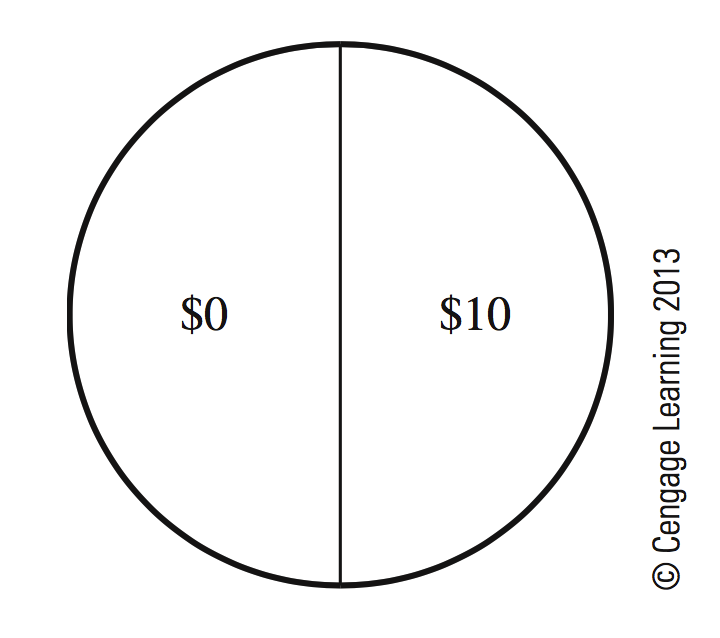
\includegraphics[height=.4\textheight{}]{9_1.png}
  \end{figure}
  
\end{frame}

\begin{frame}{Deal or No Deal?}

  \begin{itemize}
  \item<1-> 剩下两个盒子,一个\$0.01,一个\$1000000
  \item<1-> Deal: 庄家给你\$400000报酬
  \item<1-> No Deal: 继续玩
  \item<2-> $E = \$1 \times 0.5 + \$1000000 \times 0.5 \approx \$500000$
  \item<3-> 你会如何抉择?
  \end{itemize}
  
\end{frame}

\begin{frame}{修建什么样的工厂?}
  
  \begin{figure}
    \centering
    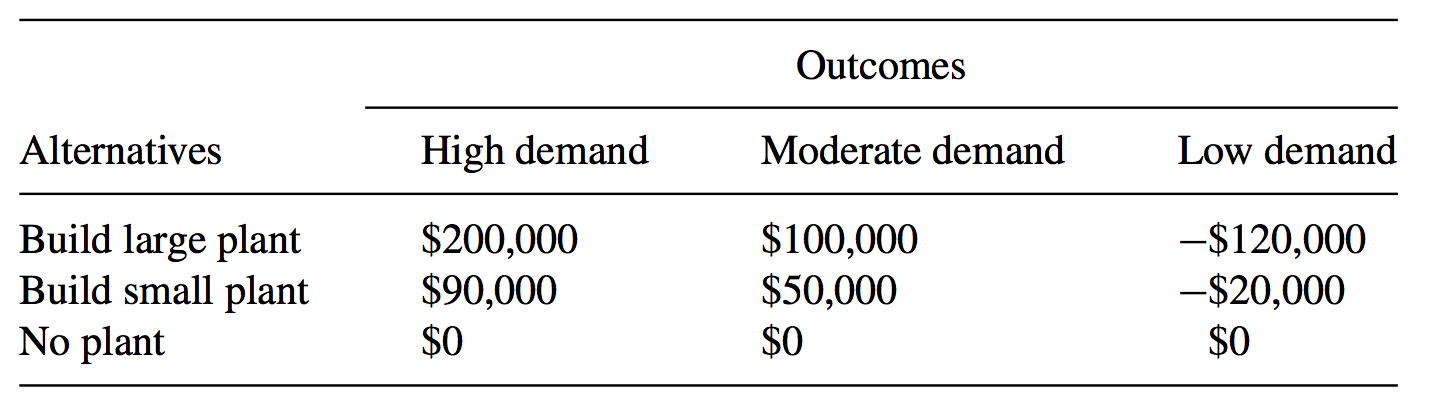
\includegraphics[width=\textwidth{}]{factories.png}
  \end{figure}

  \begin{itemize}
  \item 无法估计需求概率该如何决策?
  \item 高、中、低需求的概率分别是$25\%$、$40\%$、$35\%$决策如何改变?
  \item 这些估计是相关的频率还是专家判断?
  \item $\cdots$
  \end{itemize}

\end{frame}

\begin{frame}{概率和期望值}

  \begin{itemize}
  \item<1-> 掷出一对骰子,点数之和为7算赢
  \item<1-> \$1玩一次,赢了可以拿回\$1并另得\$5
  \item<2-> $E = \$5 \times \frac{1}{6} + (-\$1) \times \frac{5}{6} = 0$
  \item<3-> 公平游戏
  \item<4-> 如果\$2玩一次呢?
  \end{itemize}
  
  \begin{figure}
    \centering
    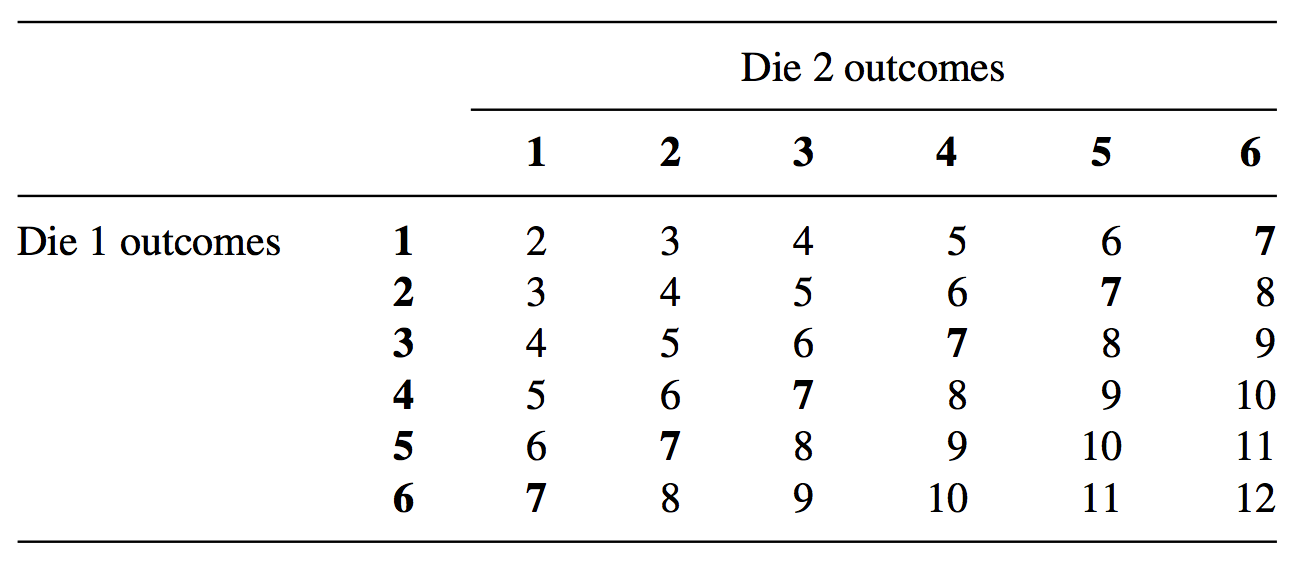
\includegraphics[width=\textwidth{}]{dice.png}
  \end{figure}
  
\end{frame}

\begin{frame}{人寿保险}

  \begin{itemize}
  \item<1-> 保险公司将一年期\$250000保单卖给49岁女性
  \item<1-> 保费\$550
  \item<1-> 49岁女性的存活率0.99791
  \item<2-> $E = \$550 \times 0.99791 - \$250000 \times (1 - 0.99791) = \$25.201$
  \end{itemize}
  
\end{frame}

\begin{frame}{高尔夫球场的改建还是新建?}

  \begin{figure}
    \centering
    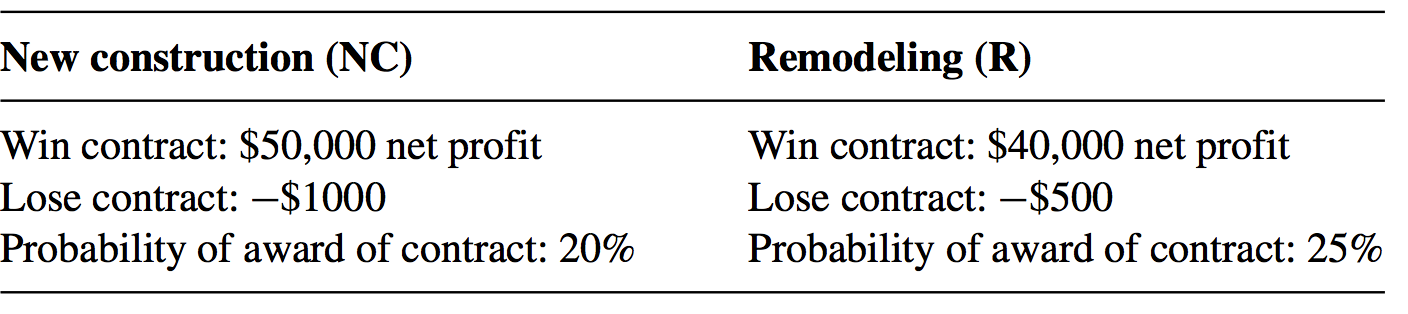
\includegraphics[width=\textwidth{}]{golf.png}
  \end{figure}
  
  \begin{itemize}
  \item<2-> $E(NC) = (\$50,000) \times 0.2 + (-\$1,000) \times 0.8 = \$9,200$
  \item<3-> $E(R) = (\$40,000) \times 0.25 + (-\$500) \times 0.75 = \$9,625$
  \item<4-> 长期来看,改建现有的高尔夫球场更赚钱
  \item<5-> 敏感性分析(赢得合同概率、利润)
  \end{itemize}
  
\end{frame}

\begin{frame}{决策树}
  
  \begin{figure}
    \centering
    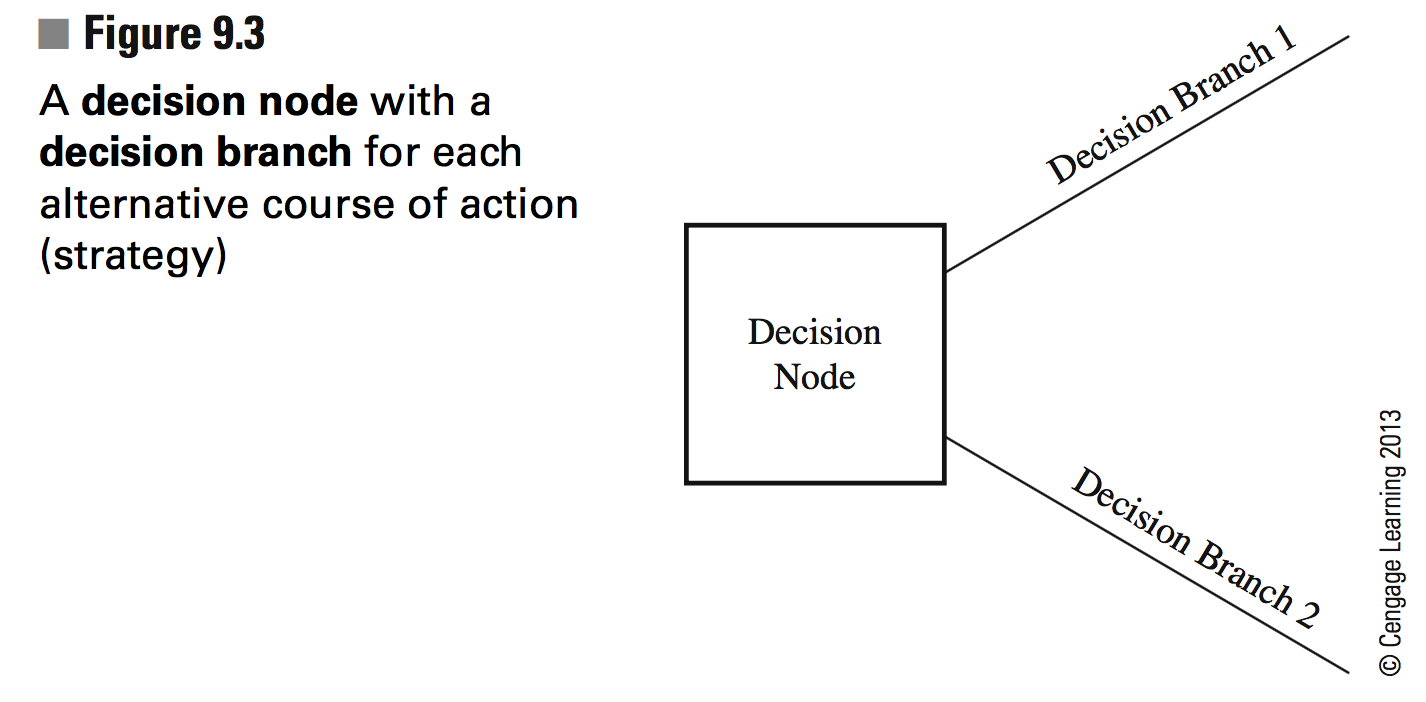
\includegraphics[width=\textwidth{}]{9_3.png}
  \end{figure}
  
\end{frame}

\begin{frame}{决策树}
  
  \begin{figure}
    \centering
    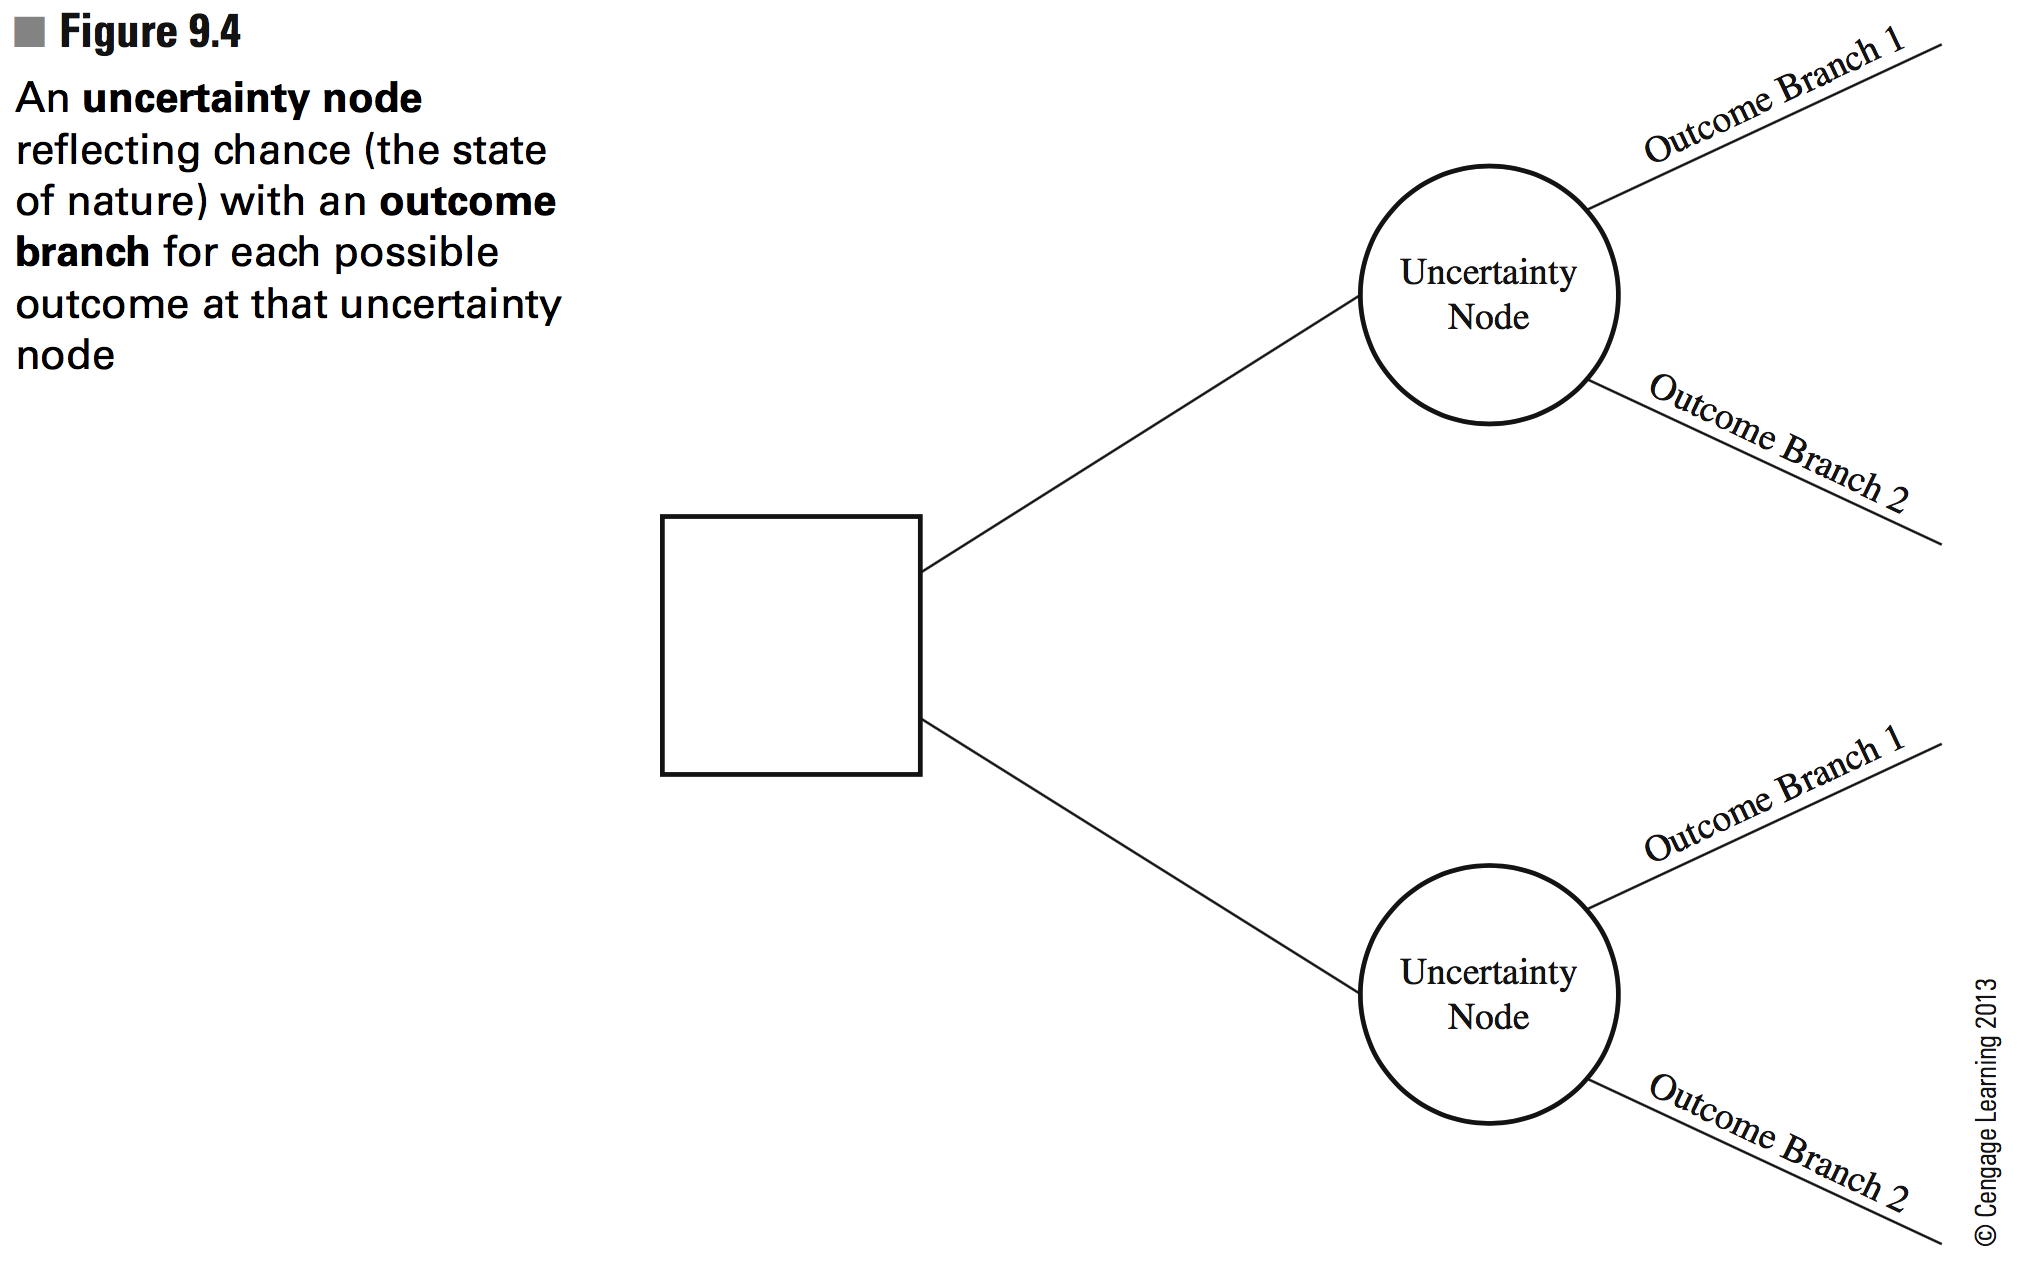
\includegraphics[width=\textwidth{}]{9_4.png}
  \end{figure}
  
\end{frame}

\begin{frame}{决策树}
  
  \begin{figure}
    \centering
    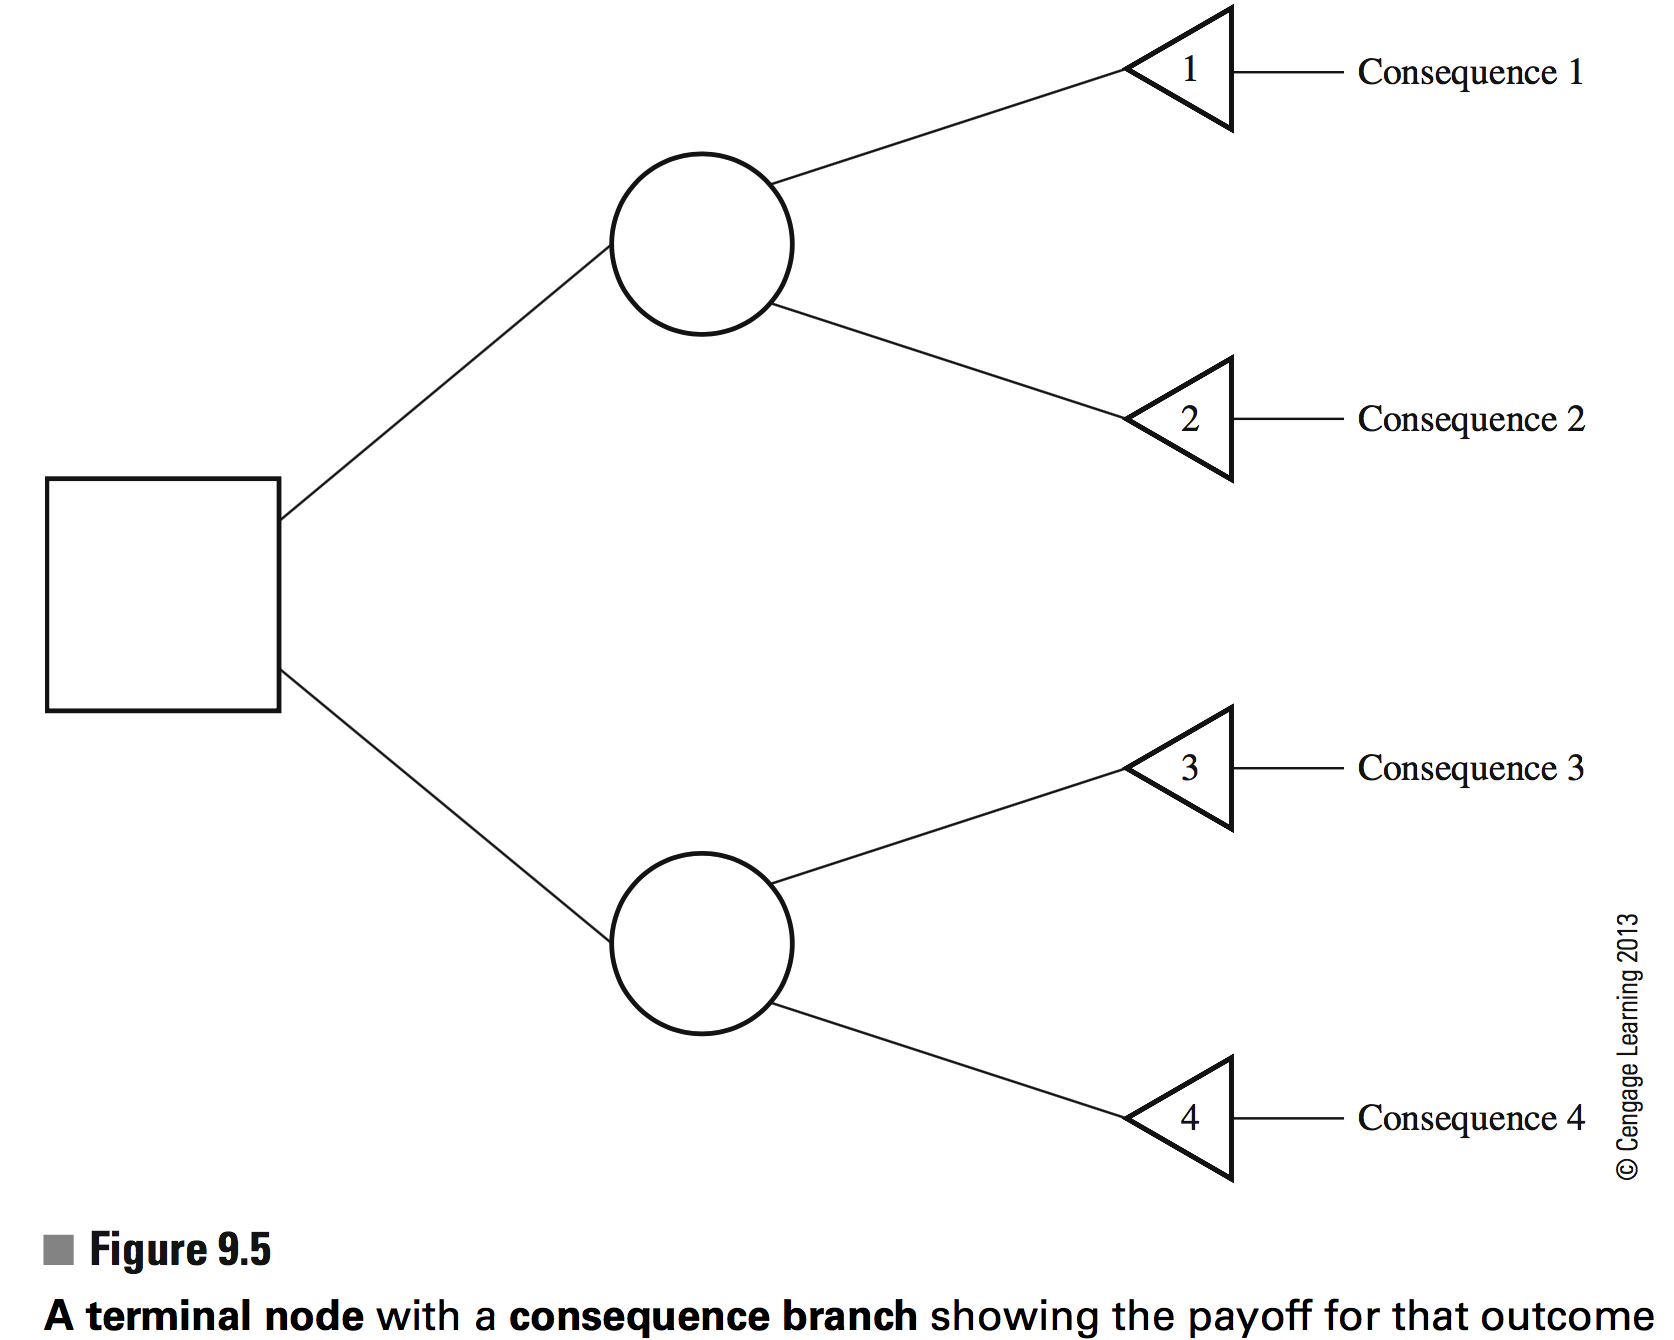
\includegraphics[width=0.8\textwidth{}]{9_5.png}
  \end{figure}
  
\end{frame}

\begin{frame}{用决策树选择新建或改建}
  
  \begin{figure}
    \centering
    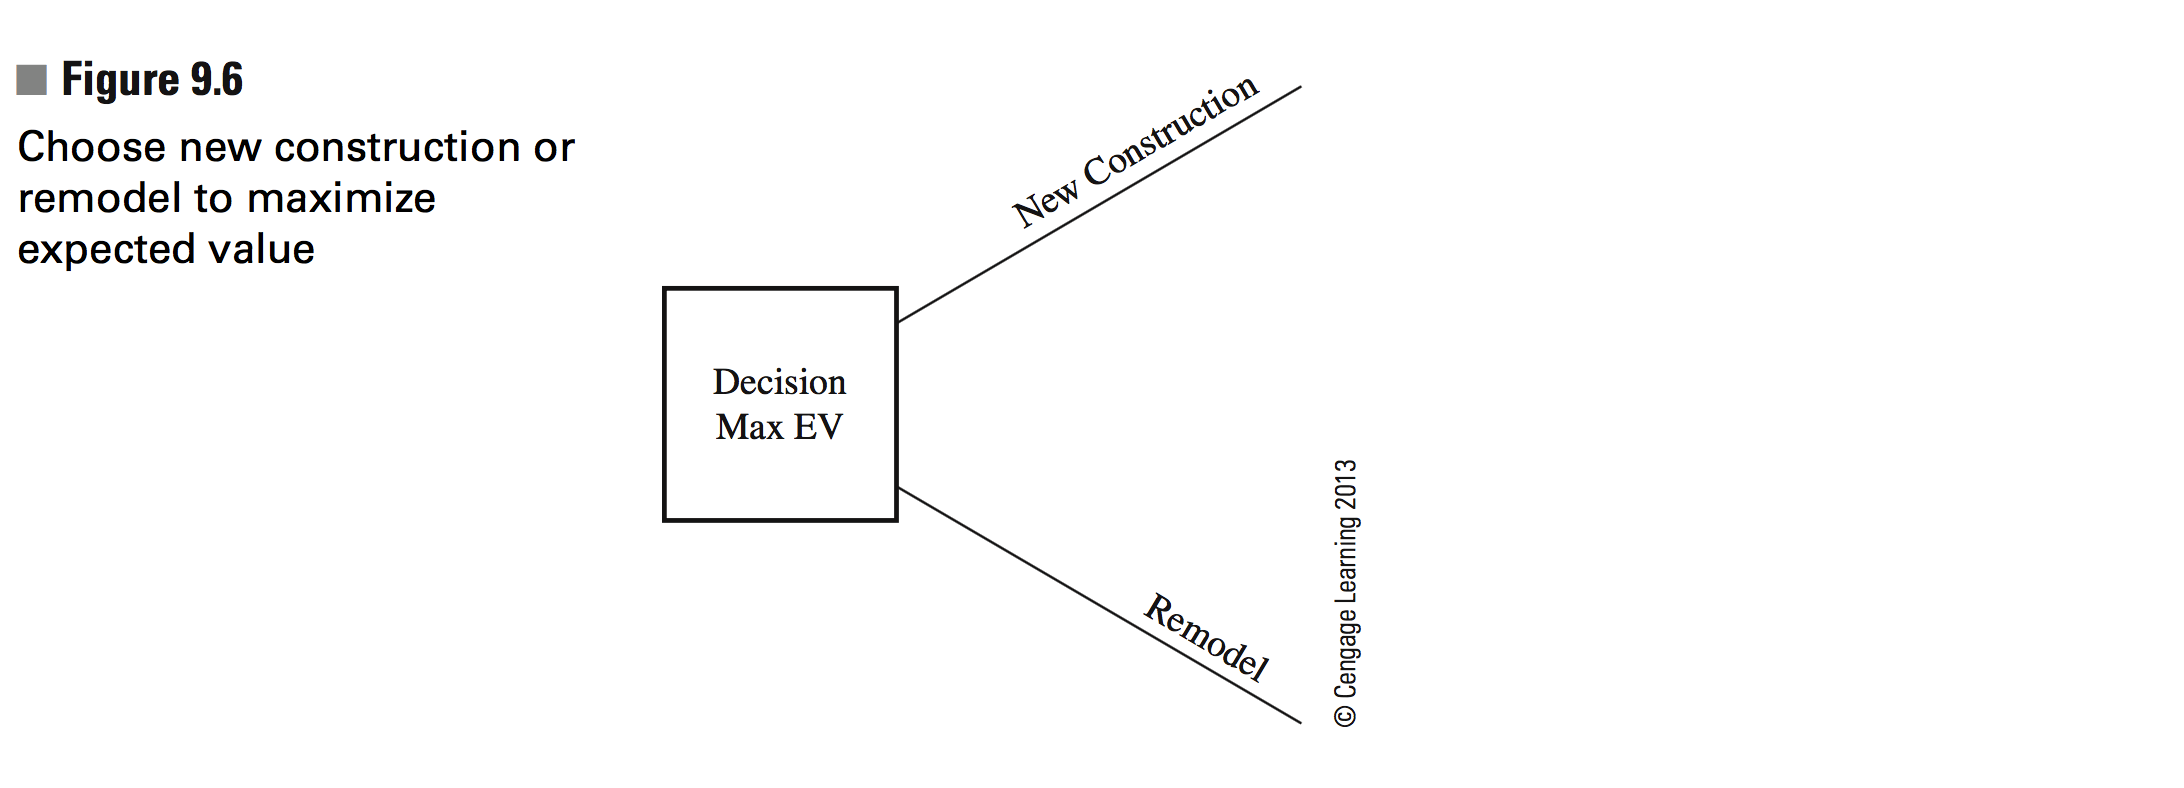
\includegraphics[width=\textwidth{}]{9_6.png}
  \end{figure}

\end{frame}

\begin{frame}{用决策树选择新建或改建}
  
  \begin{figure}
    \centering
    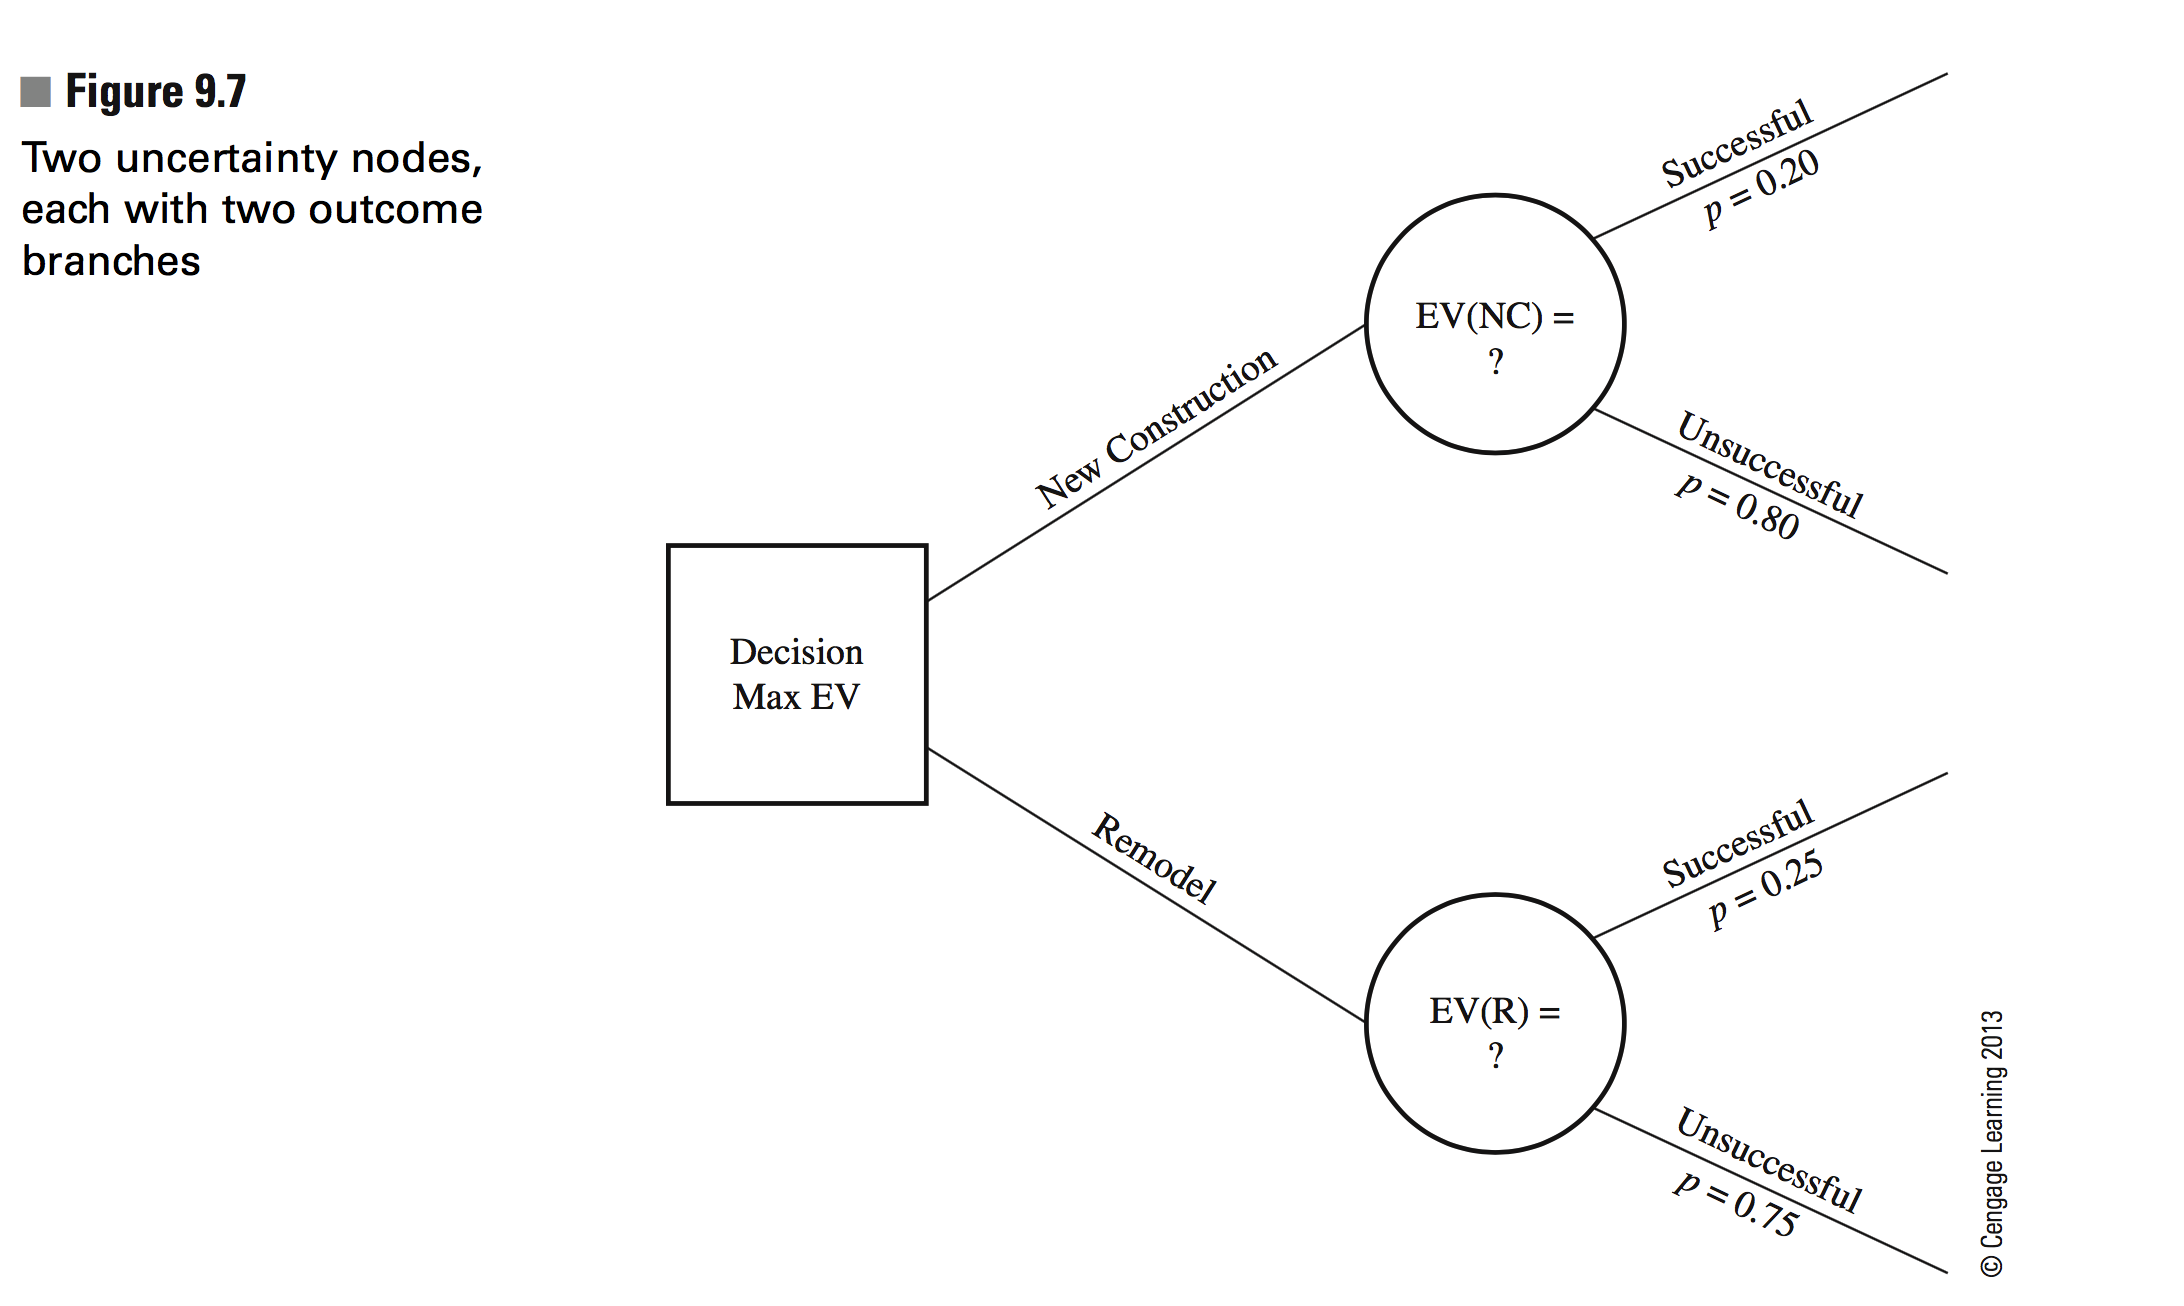
\includegraphics[width=\textwidth{}]{9_7.png}
  \end{figure}

\end{frame}

\begin{frame}{用决策树选择新建或改建}
  
  \begin{figure}
    \centering
    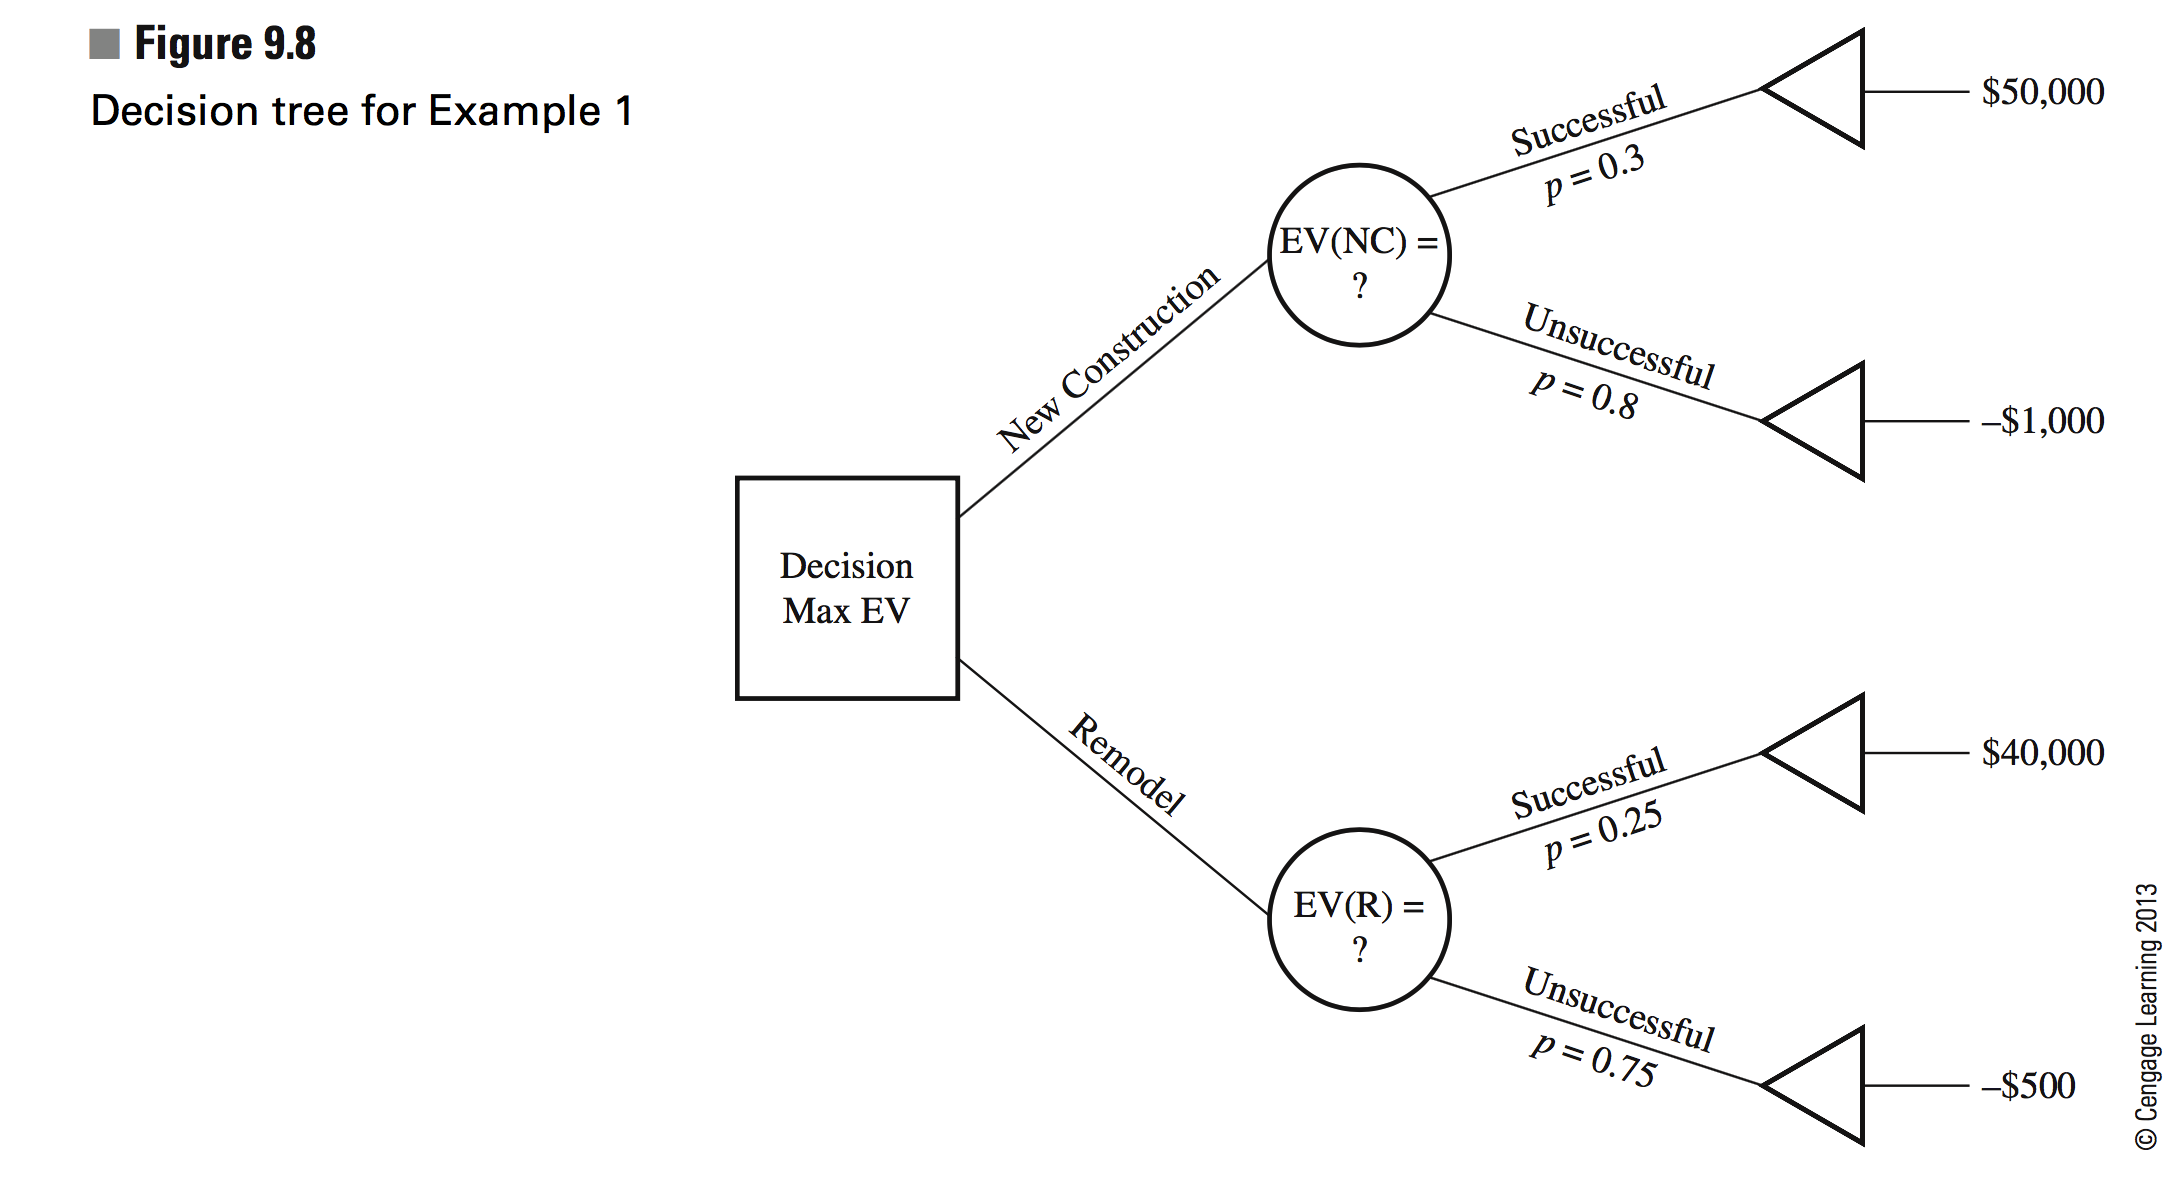
\includegraphics[width=\textwidth{}]{9_8.png}
  \end{figure}

\end{frame}

\begin{frame}{用决策树选择新建或改建}
  
  \begin{figure}
    \centering
    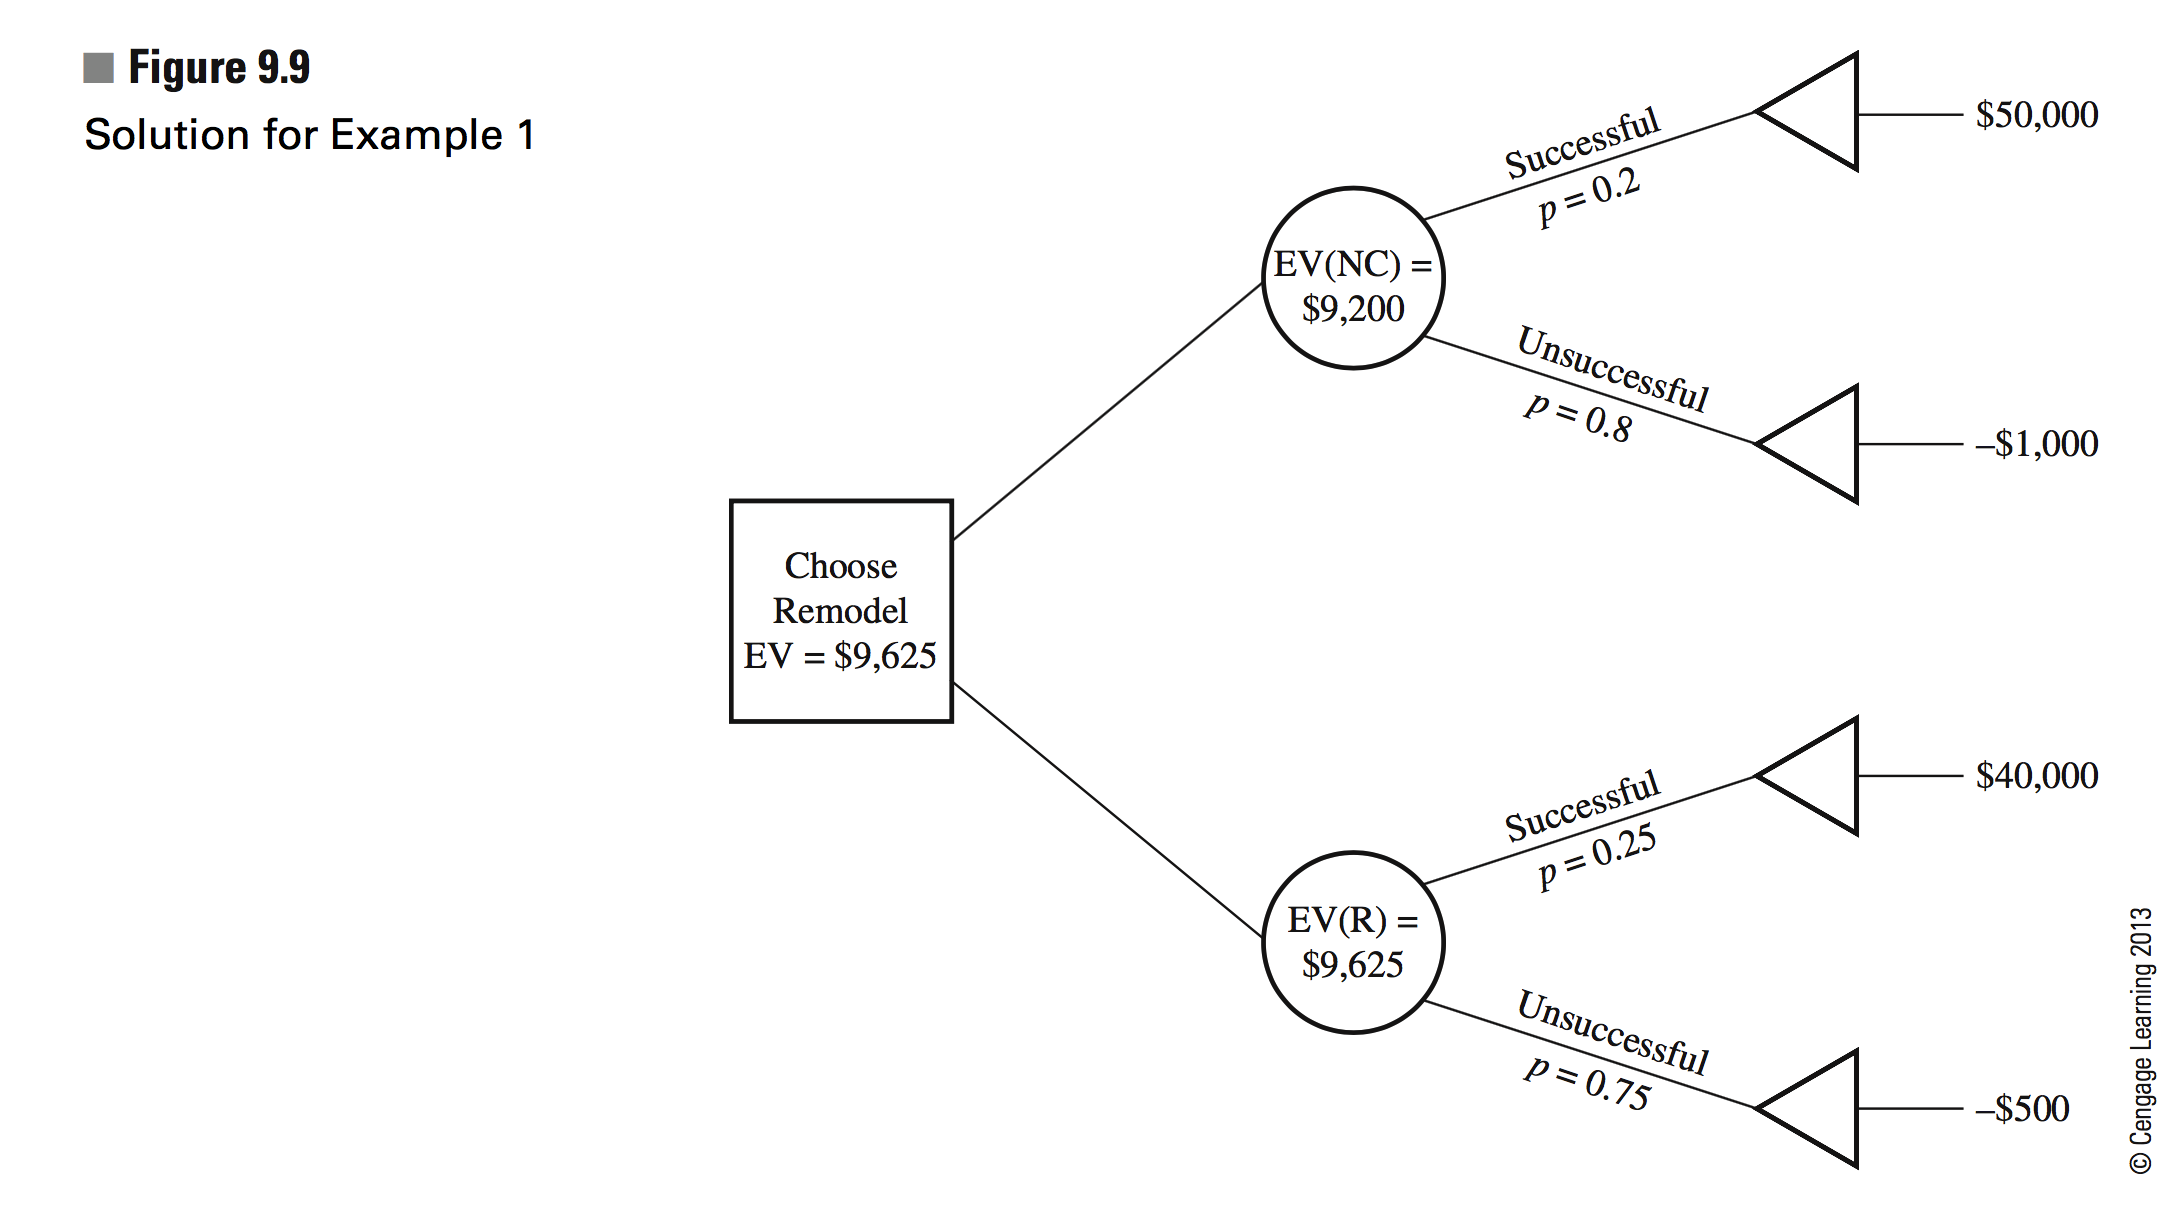
\includegraphics[width=\textwidth{}]{9_9.png}
  \end{figure}

\end{frame}

\begin{frame}{折返方法}
  
  \begin{figure}
    \centering
    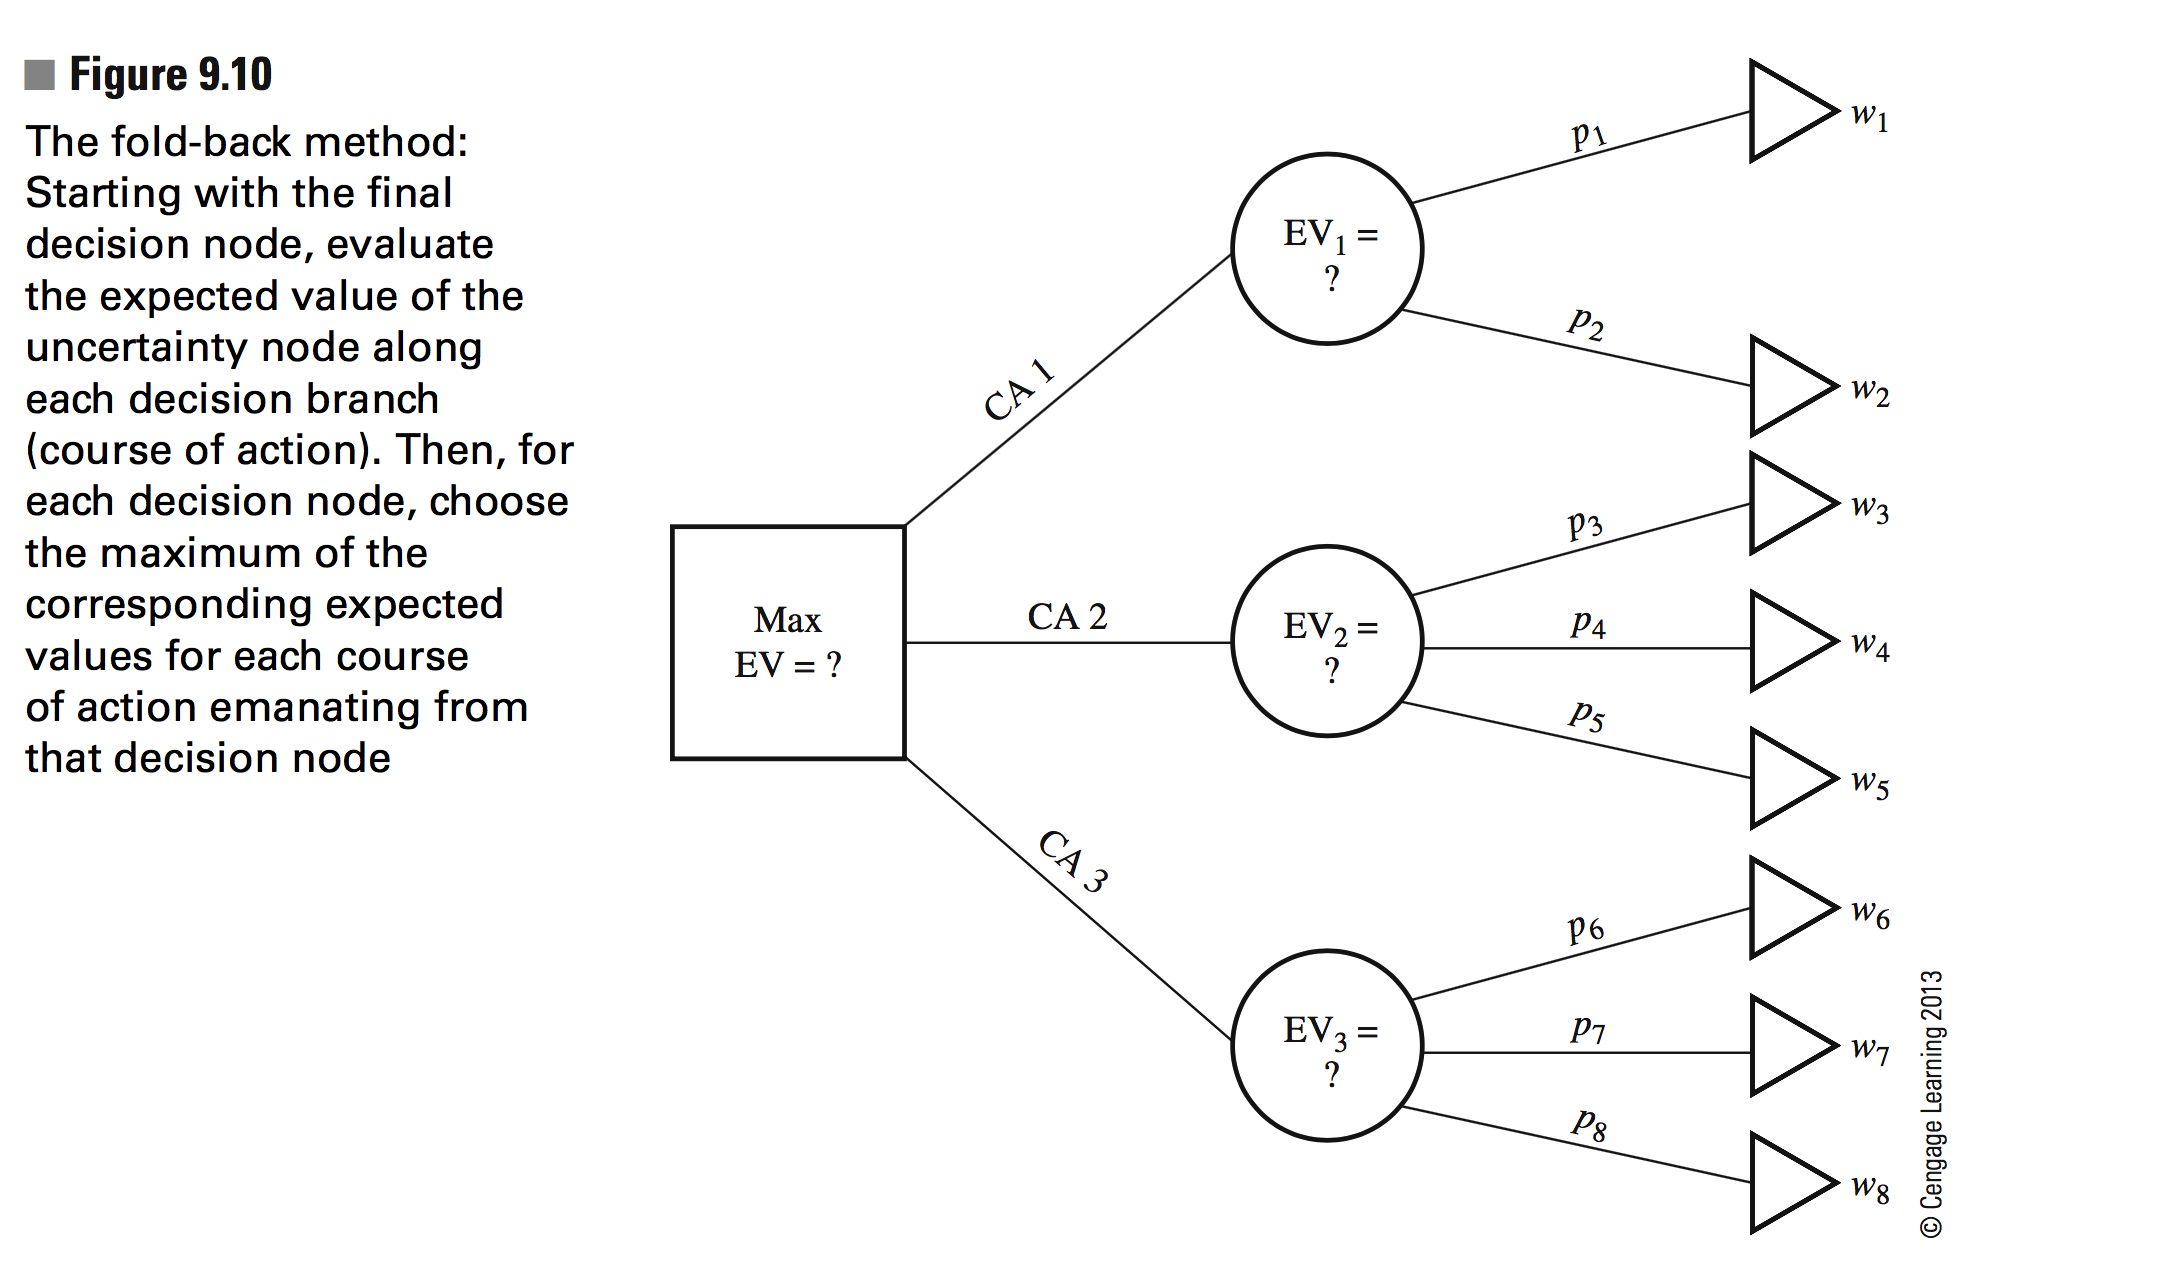
\includegraphics[width=\textwidth{}]{9_10.png}
  \end{figure}

\end{frame}

\begin{frame}{Hardware \& Lumber公司的决策}
  
  \begin{figure}
    \centering
    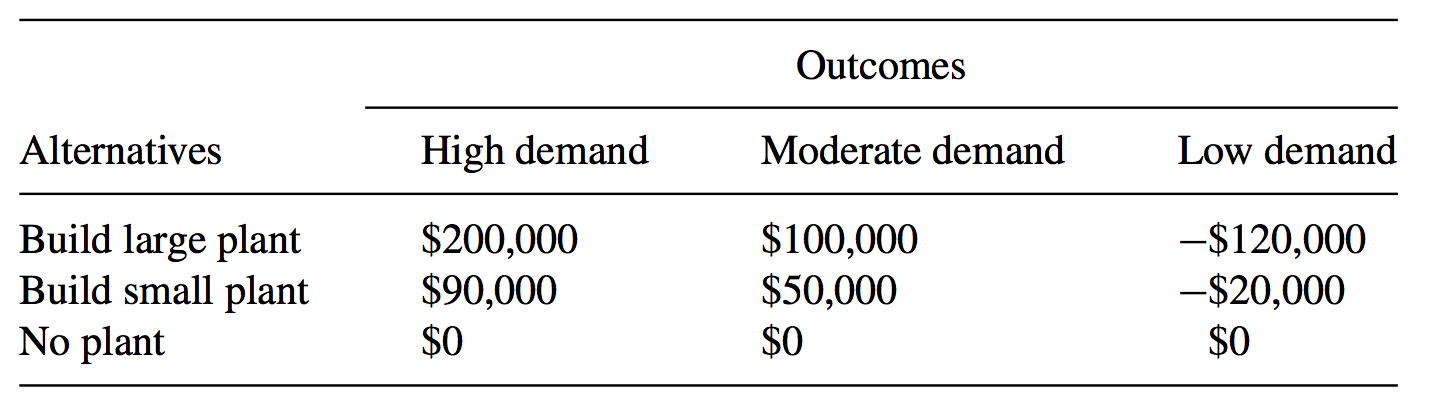
\includegraphics[width=\textwidth{}]{factories.png}
  \end{figure}

\end{frame}

\begin{frame}{Hardware \& Lumber公司的决策}
  
  \begin{figure}
    \centering
    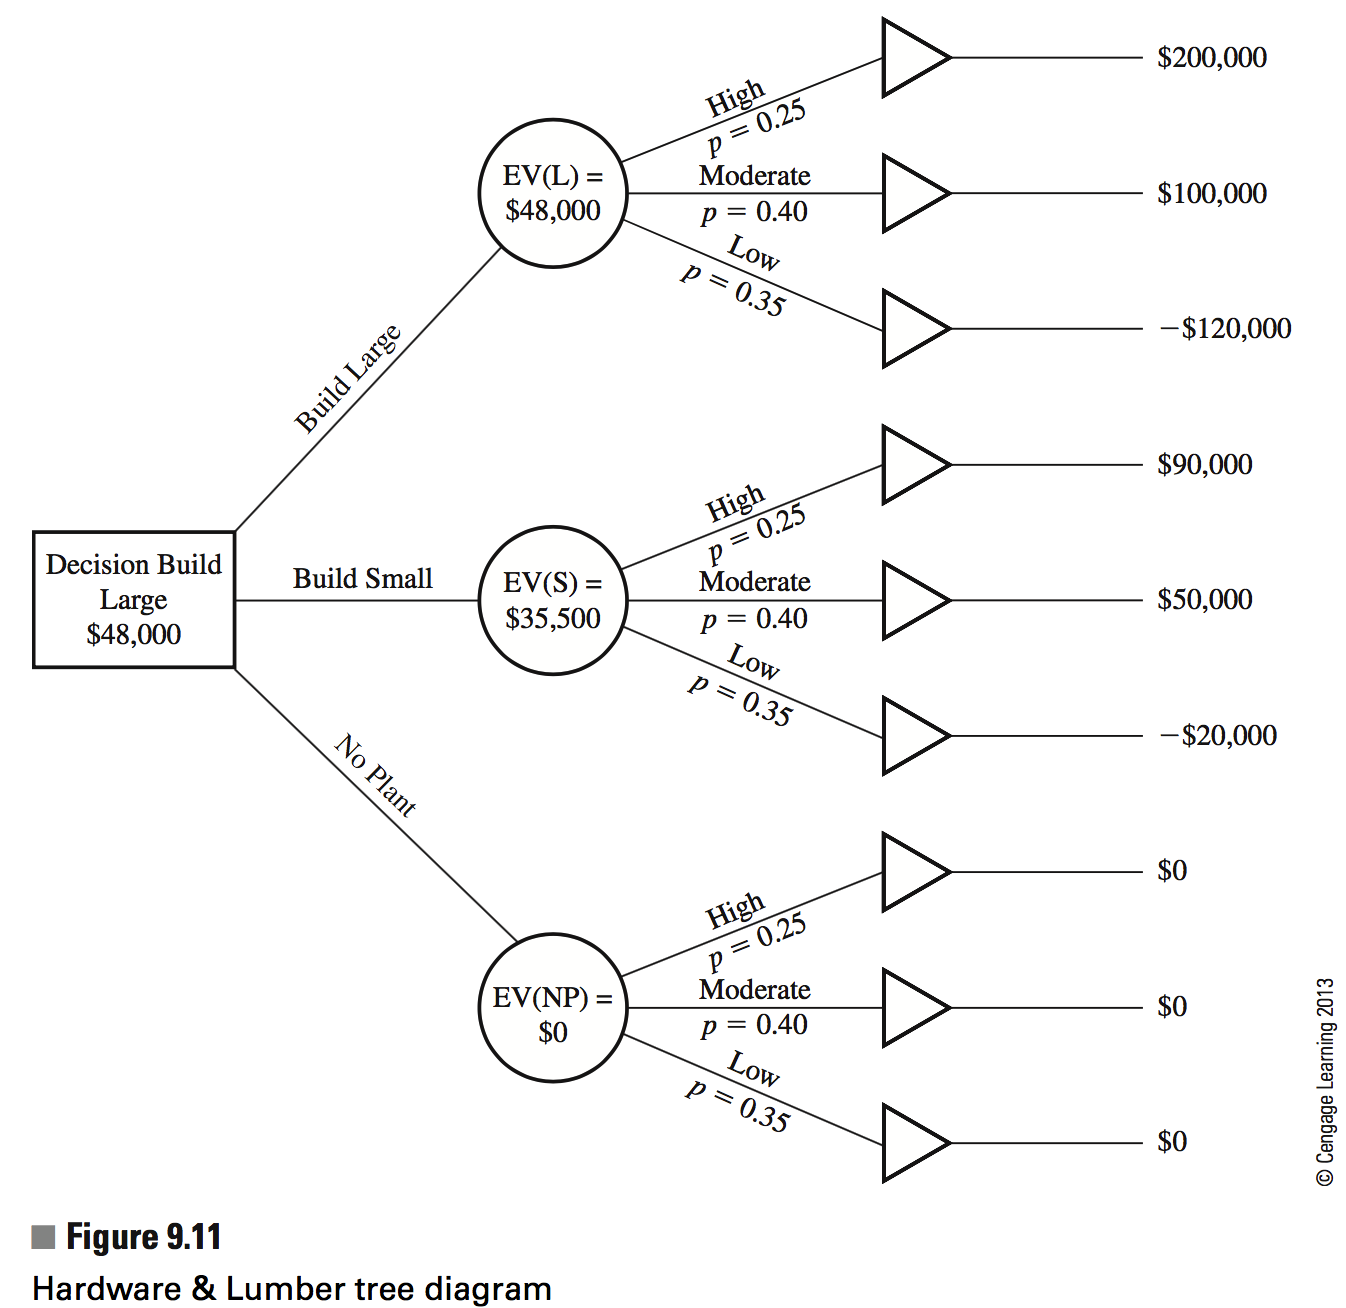
\includegraphics[height=0.8\textheight{}]{9_11.png}
  \end{figure}

\end{frame}

\begin{frame}{地方电视台}
  
  \begin{figure}
    \centering
    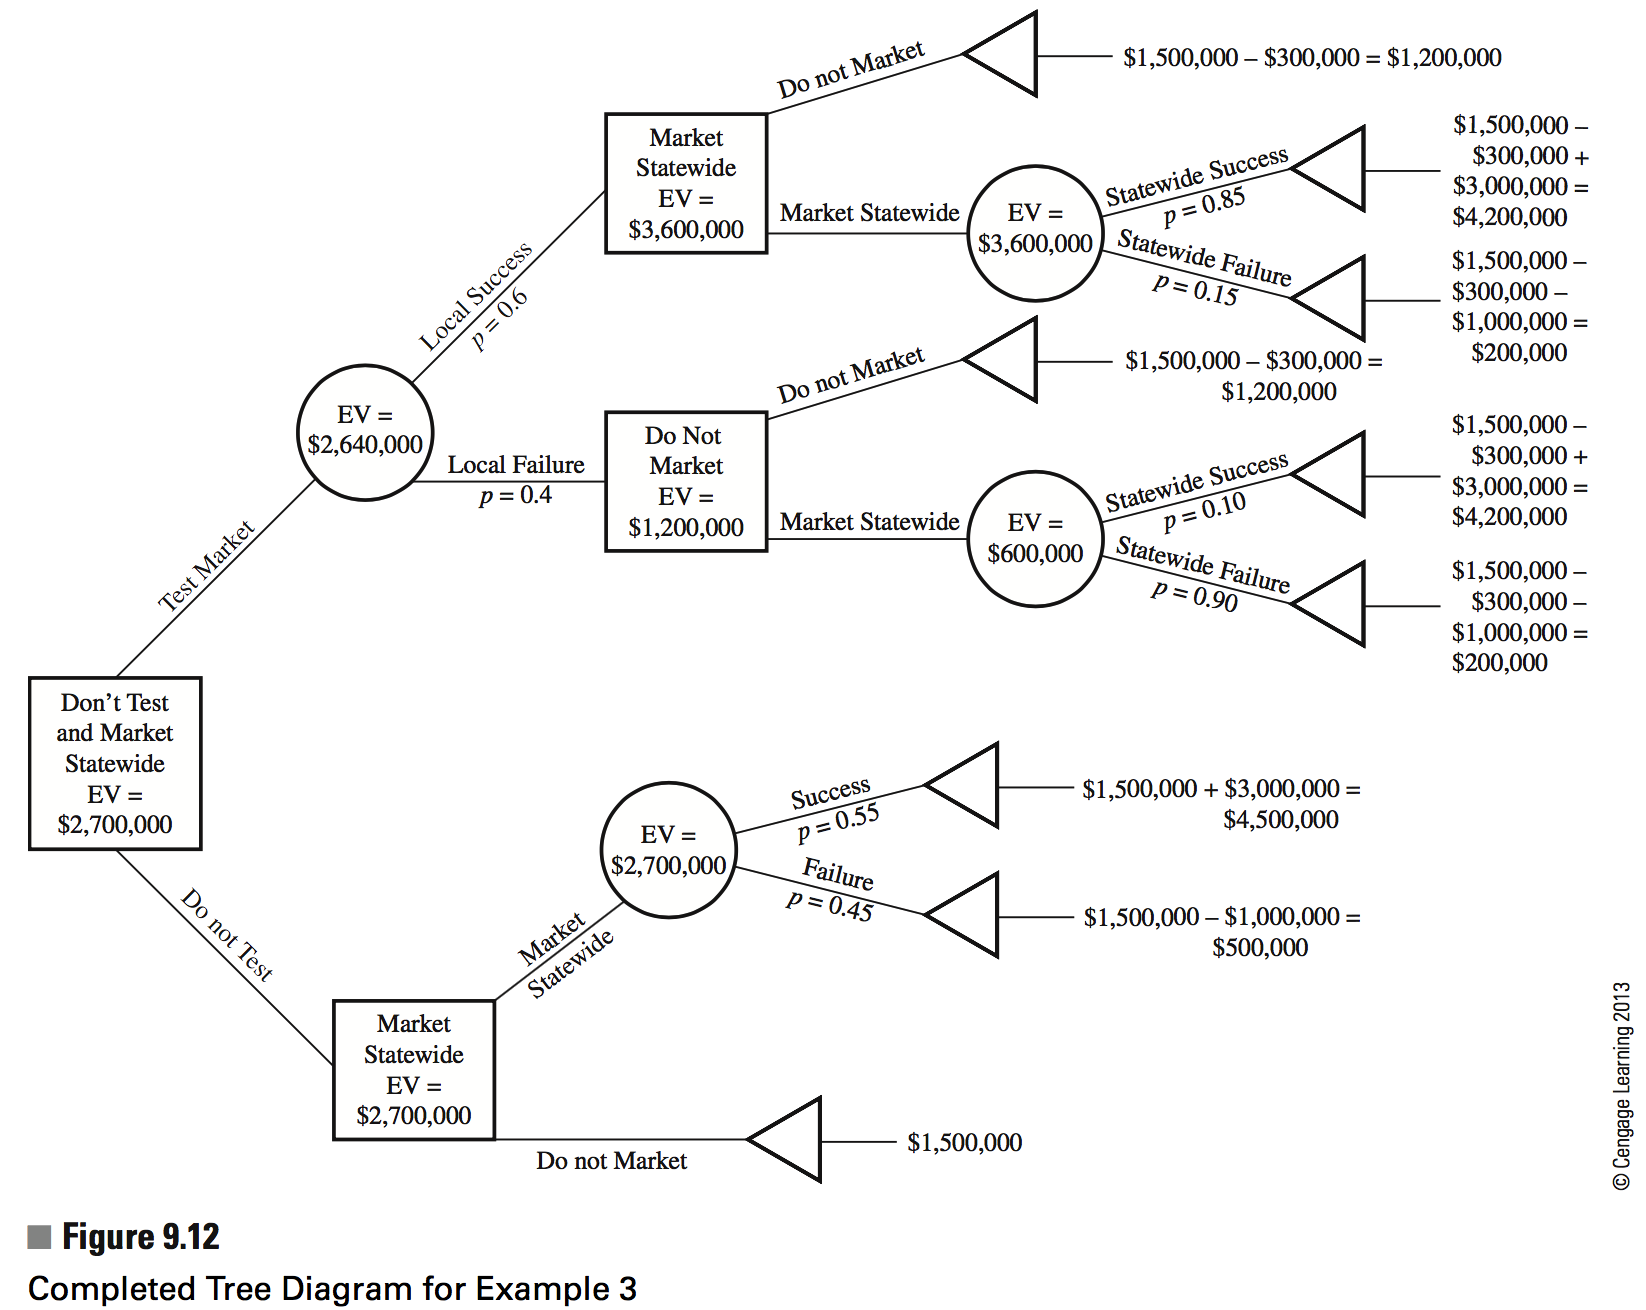
\includegraphics[height=0.8\textheight{}]{9_12.png}
  \end{figure}

\end{frame}

\begin{frame}{序列决策和条件概率}
  
  \begin{figure}
    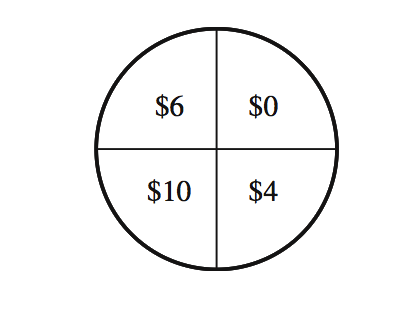
\includegraphics[height=0.4\textheight{}]{lunpan.png}
    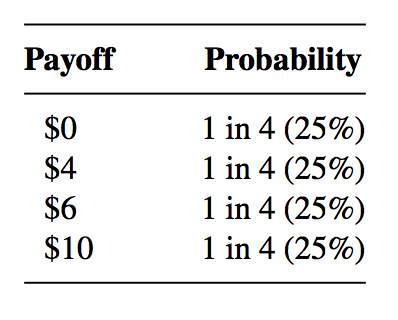
\includegraphics[height=0.4\textheight{}]{payoff.png}
  \end{figure}

  \begin{itemize}
  \item 每盘游戏可以转3次,随时可以停止,寻求最优策略
  \end{itemize}

\end{frame}

\begin{frame}{序列决策和条件概率}
  
  \begin{figure}
    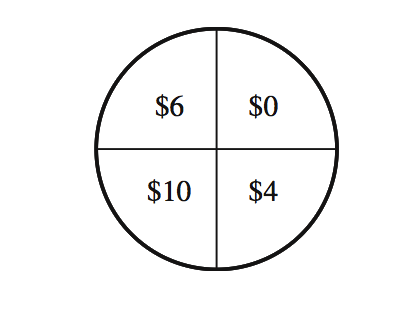
\includegraphics[height=0.4\textheight{}]{lunpan.png}
    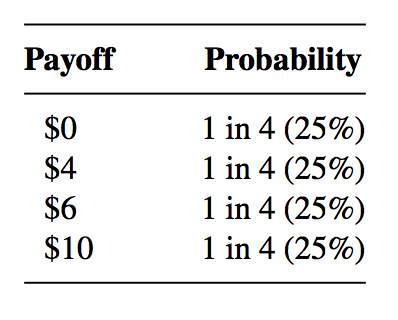
\includegraphics[height=0.4\textheight{}]{payoff.png}
  \end{figure}

  \begin{itemize}
  \item<1-> $E(3) = \$10 \times 0.25 + \$6 \times 0.25 + \$4 \times 0.25 + \$0 \times 0.25 = \$5.00$
  \item<2-> $E(2) = \$10 \times 0.25 + \$6 \times 0.25 + \$5 \times 0.5 = \$6.50$
  \item<3-> $E(1) = \$10 \times 0.25 + \$6.5 \times 0.75 \approx \$7.375$
  \end{itemize}

\end{frame}

\begin{frame}{序列决策和条件概率}
  
  \begin{figure}
    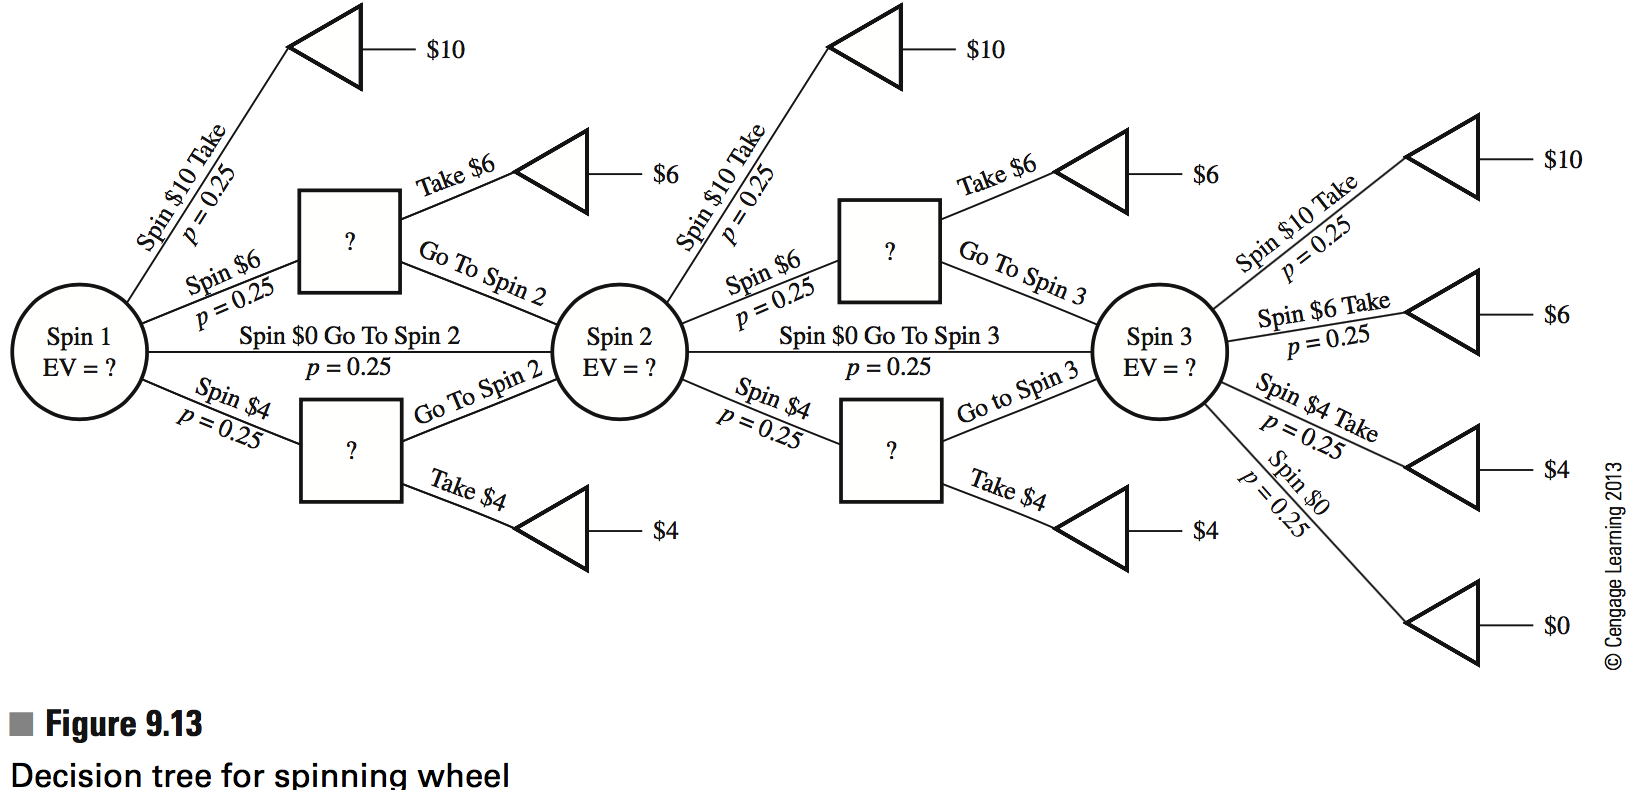
\includegraphics[width=\textwidth{}]{9_13.png}
  \end{figure}

\end{frame}

\begin{frame}{序列决策和条件概率}
  
  \begin{figure}
    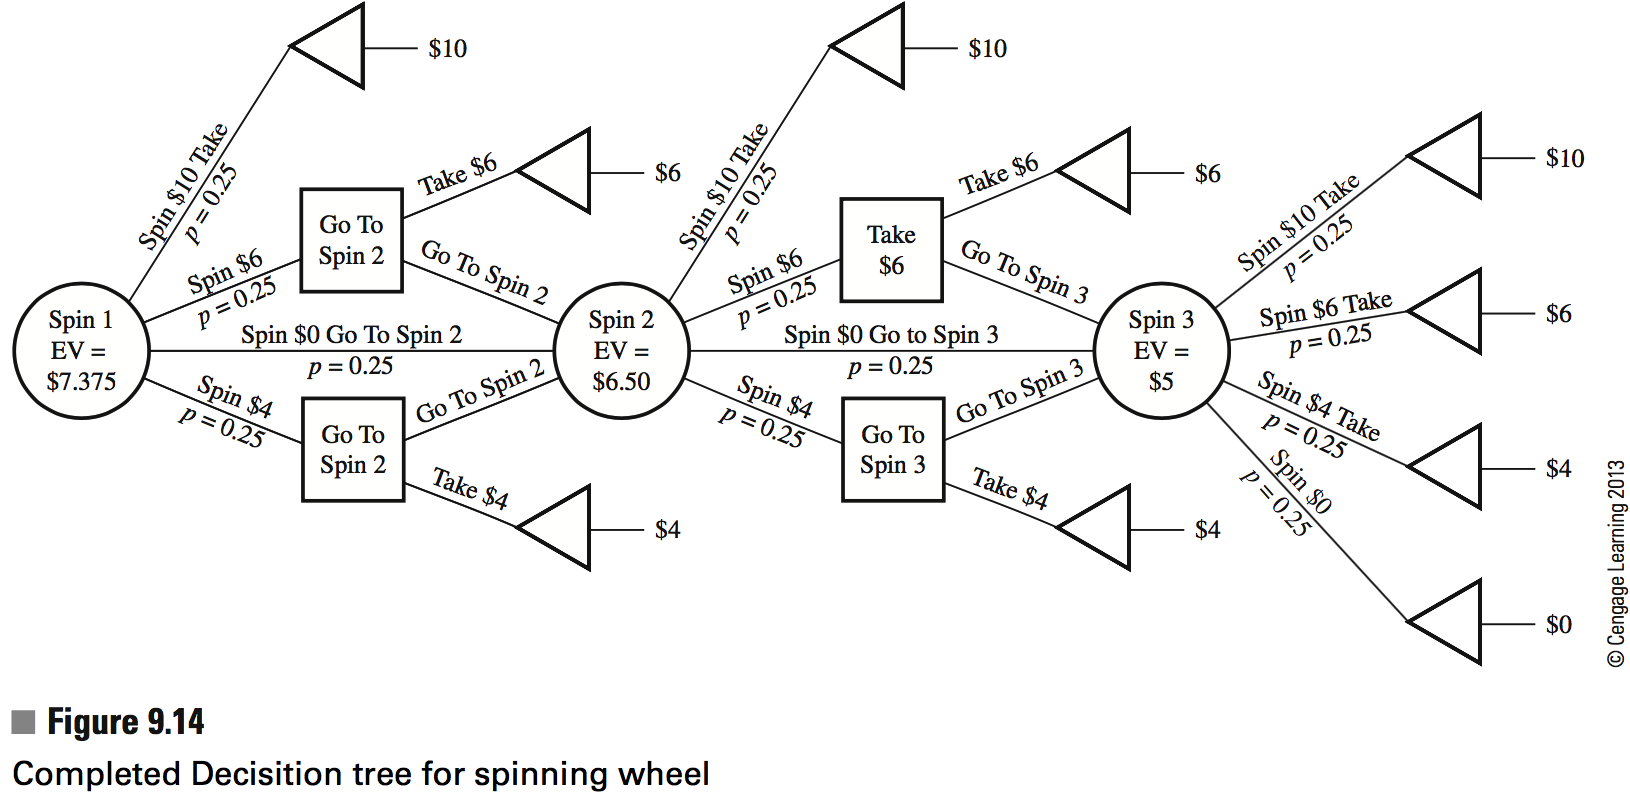
\includegraphics[width=\textwidth{}]{9_14.png}
  \end{figure}

\end{frame}

\begin{frame}{再论Hardware \& Lumber公司的决策}
  
  \begin{figure}
    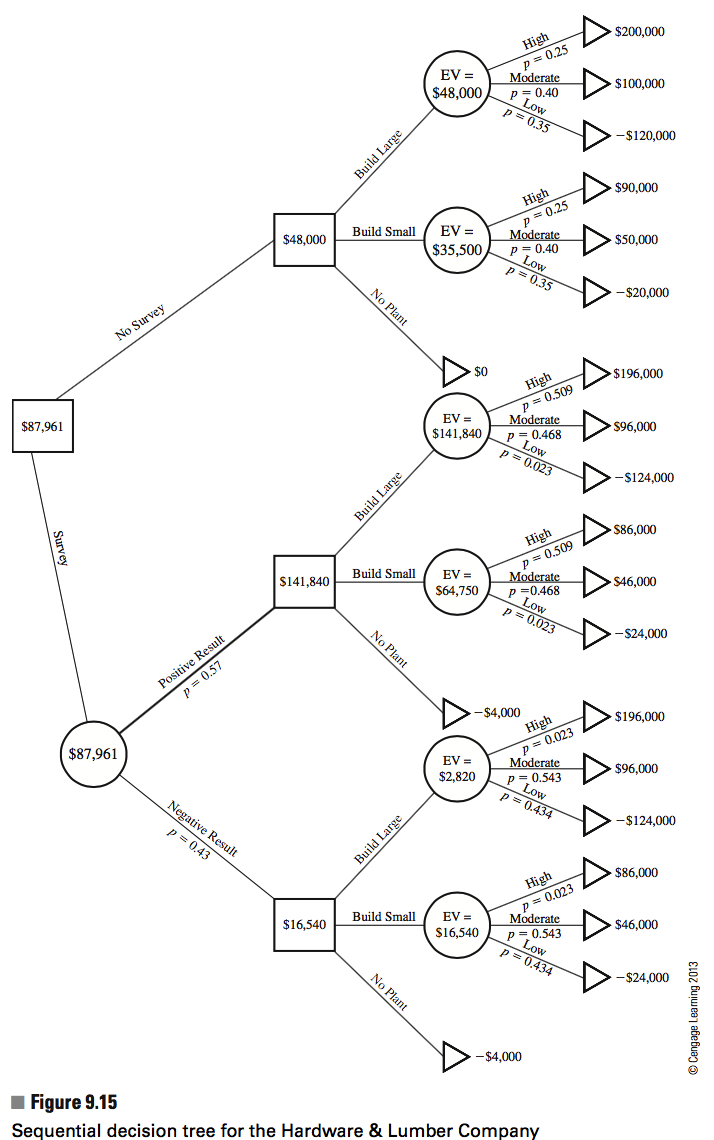
\includegraphics[height=0.8\textheight{}]{9_15.png}
  \end{figure}

\end{frame}

\begin{frame}{类固醇的检测}
  
  \begin{figure}
    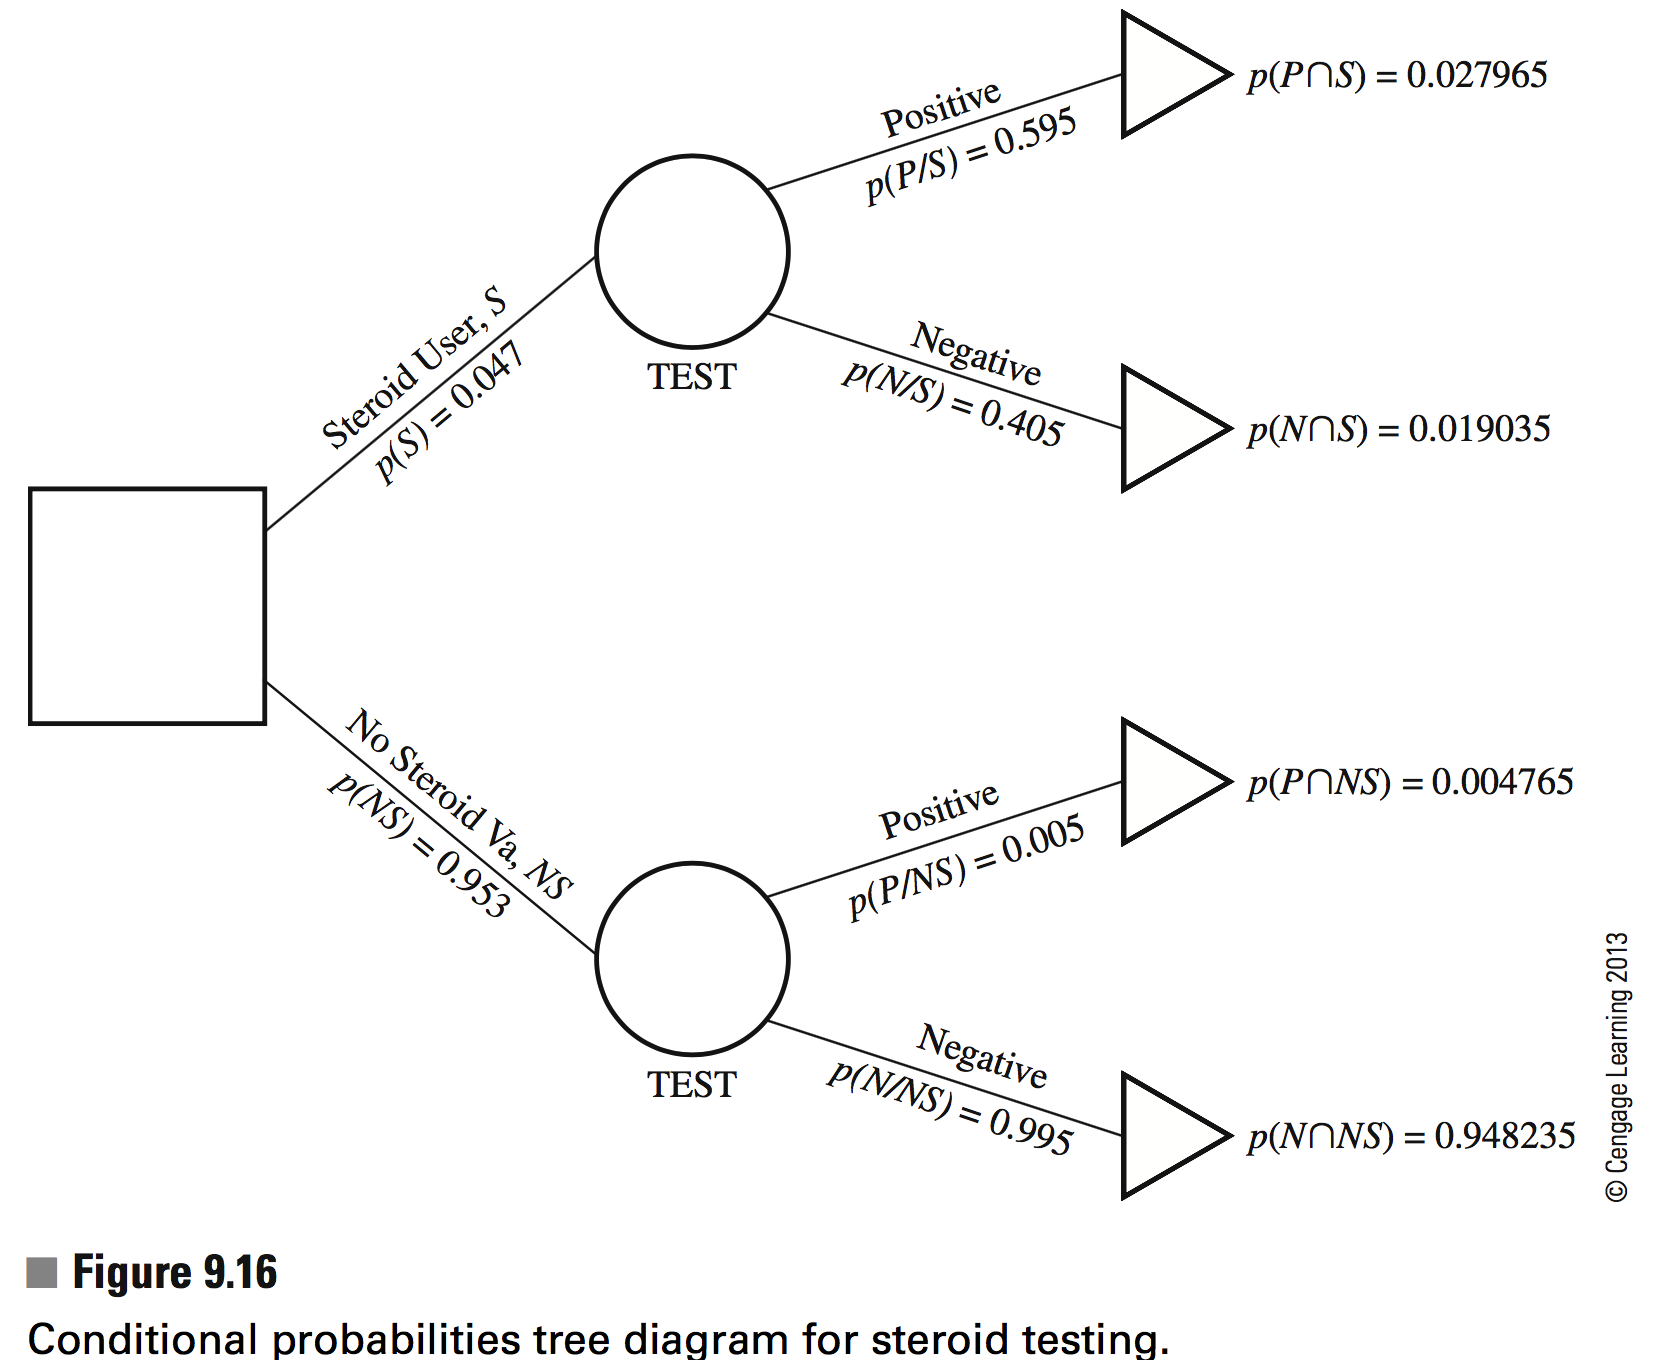
\includegraphics[width=0.8\textwidth{}]{9_16.png}
  \end{figure}

\end{frame}

\begin{frame}{利用各种准则的决策}

  \begin{itemize}
  \item 风险
  \item 一次性决策与长期决策
  \end{itemize}
  
\end{frame}

\begin{frame}{投资与状态}

  \begin{itemize}
  \item 初始投资\$100000在5年后的资金(单位\$100000)
  \end{itemize}
  
  \begin{figure}
    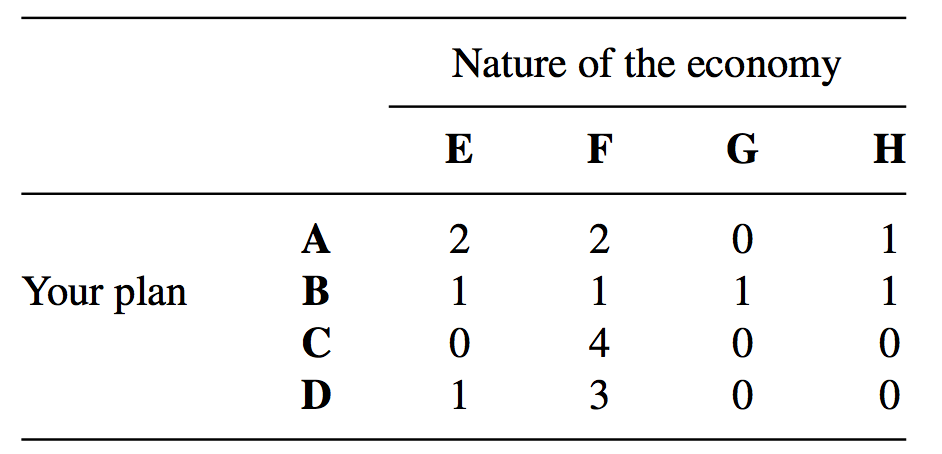
\includegraphics[width=0.8\textwidth{}]{plan.png}
  \end{figure}

\end{frame}

\begin{frame}{情形1:概率已知,最大化期望值}
  \begin{itemize}
  \item<1-> 最大化期望值准则
  \item<1-> 假设E、F、G、H的概率分别是0.2、0.4、0.3、0.1
  \item<2-> E(A) = 1.3, E(B) = 1.0, {\color{red} E(C) = 1.6}, E(D) = 1.4
  \item<3-> 不反映包含的风险, 但对一次性决策仍然有合适准则的情况
  \item<4-> 例如:某人有{\color{red} 一次性}的机会靠只{\color{red} 投掷一次}一对骰子的办法去赢\$1000
  \end{itemize}
  
\end{frame}

\begin{frame}{情形2:一次性决策,概率未知}

  \begin{description}
  \item[拉普拉斯准则] 假定未知概率都是相等的
  \item[最大最小准则] 选取具有最高下限的策略(保守策略)
  \item[最大最大准则] 乐观策略
  \item[乐观系数准则] x(row max) + (1-x)(row min),乐观、保守相结合
  \end{description}
  
\end{frame}

\begin{frame}{情形3:“费用”最小化}

  \begin{description}
  \item[最小最大准则] 选取上限最小的
  \item[最小最大缺憾准则] 使最大缺憾尽可能小
  \end{description}
  
  \begin{figure}
    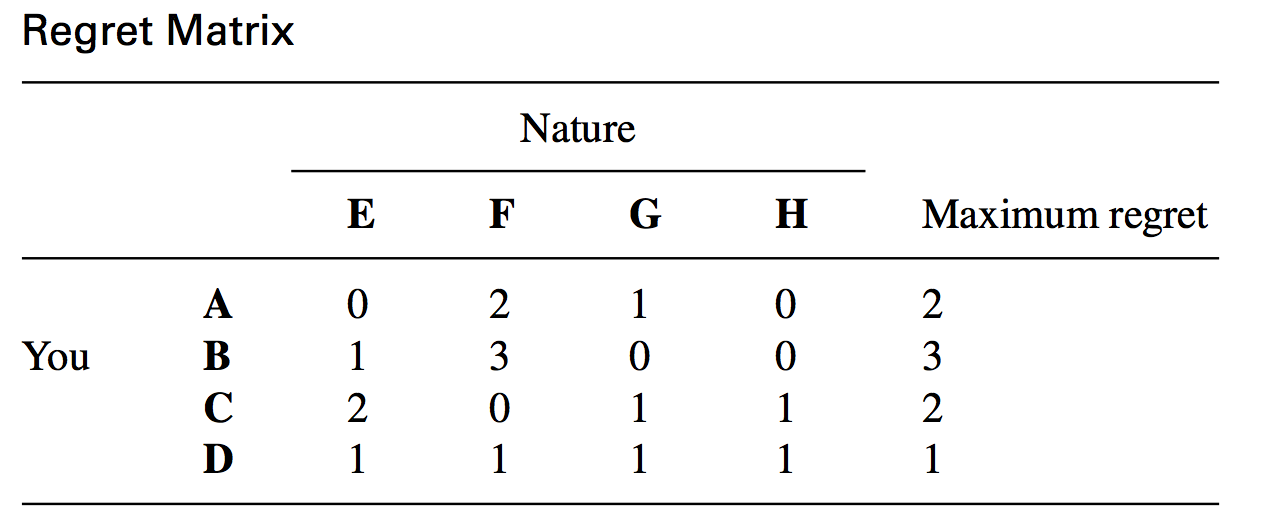
\includegraphics[width=0.8\textwidth{}]{regret.png}
  \end{figure}

\end{frame}

\begin{frame}{投资策略}
  
  \begin{figure}
    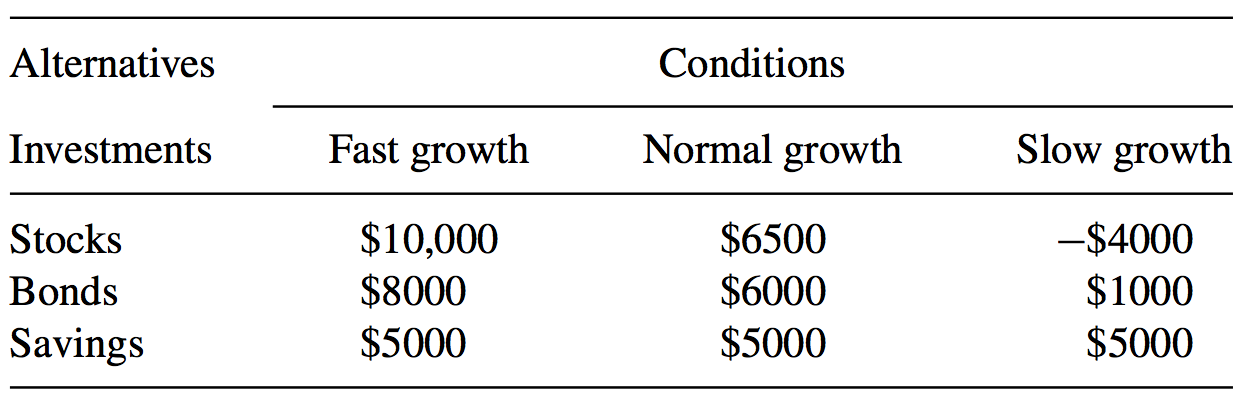
\includegraphics[width=0.8\textwidth{}]{invest.png}
  \end{figure}
  
\end{frame}

\begin{frame}{博弈论}
  
  \begin{figure}
    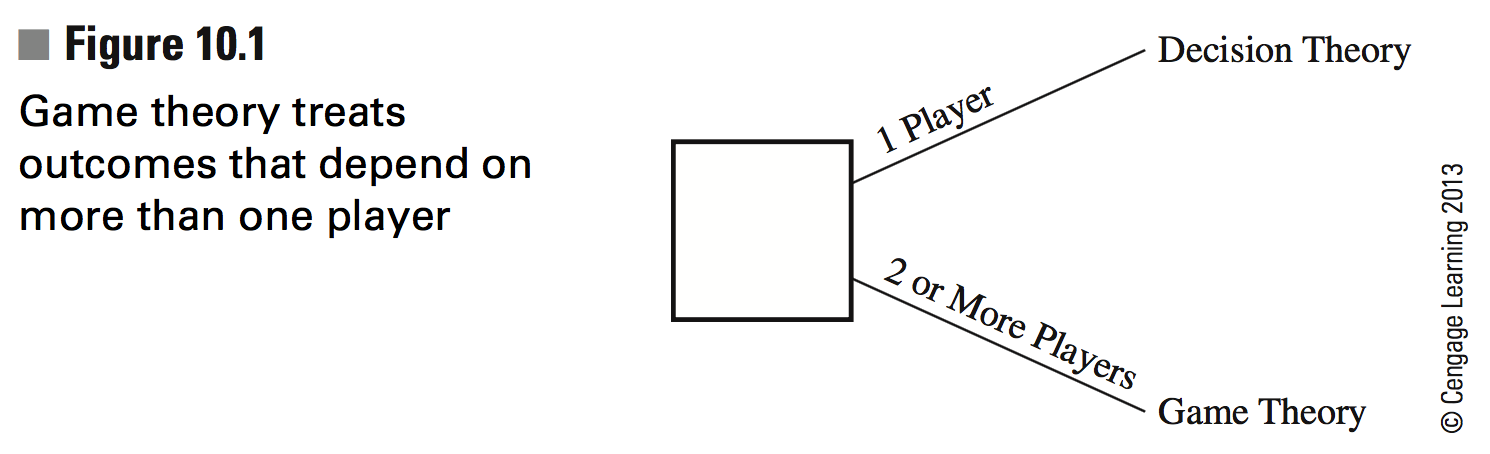
\includegraphics[width=0.8\textwidth{}]{10_1.png}
  \end{figure}

\end{frame}

\begin{frame}{五金连锁店}
  
  \begin{figure}
    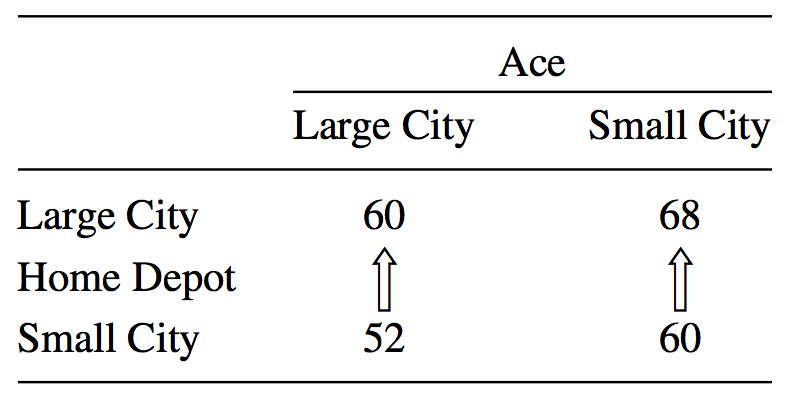
\includegraphics[width=0.8\textwidth{}]{homedepot.png}
  \end{figure}

\end{frame}

\begin{frame}{五金连锁店}
  
  \begin{figure}
    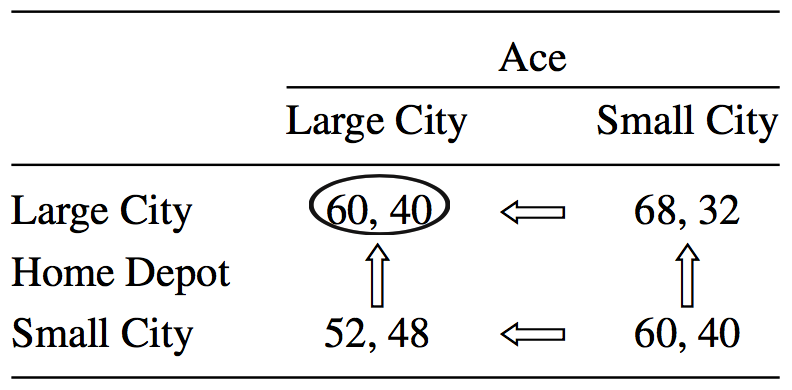
\includegraphics[width=0.8\textwidth{}]{homeace.png}
  \end{figure}

\end{frame}

\begin{frame}{纳什均衡}

  \begin{block}{纳什均衡}
   纳什均衡是这样一种结果,其中任何一个参与者都不可能通过单方面偏离与该结果想对
   应的策略获得好处。 
  \end{block}
  
\end{frame}

\begin{frame}{混合策略完全冲突博弈:投球手和击球手的较量}

  \begin{figure}
    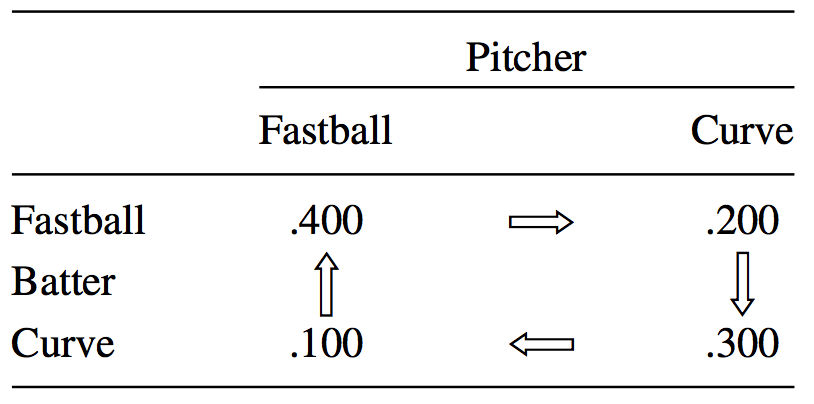
\includegraphics[width=0.8\textwidth{}]{baseball.png}
  \end{figure}
  
\end{frame}

\begin{frame}{博弈论:部分冲突}

  \begin{itemize}
  \item 囚徒困境
  \end{itemize}

  \begin{figure}
    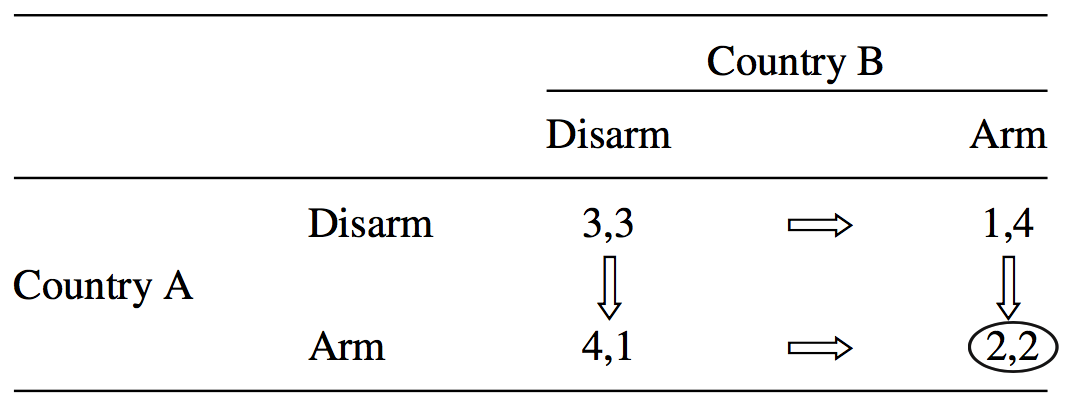
\includegraphics[width=0.8\textwidth{}]{country.png}
  \end{figure}
  
\end{frame}

\begin{frame}{完全冲突与部分冲突}
  
  \begin{figure}
    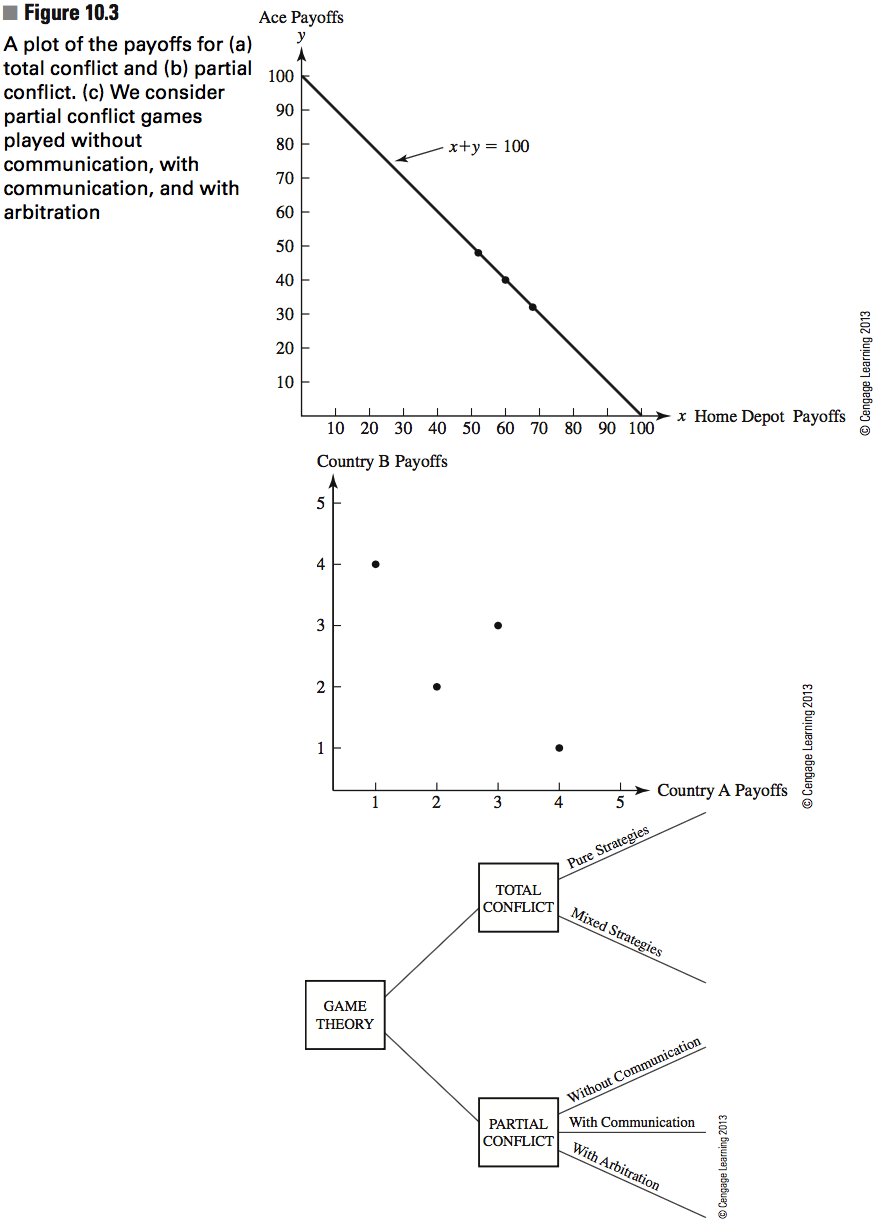
\includegraphics[height=0.8\textheight{}]{game.png}
  \end{figure}

\end{frame}

\begin{frame}{完全冲突博弈的线性规划模型}
  
  \begin{figure}
    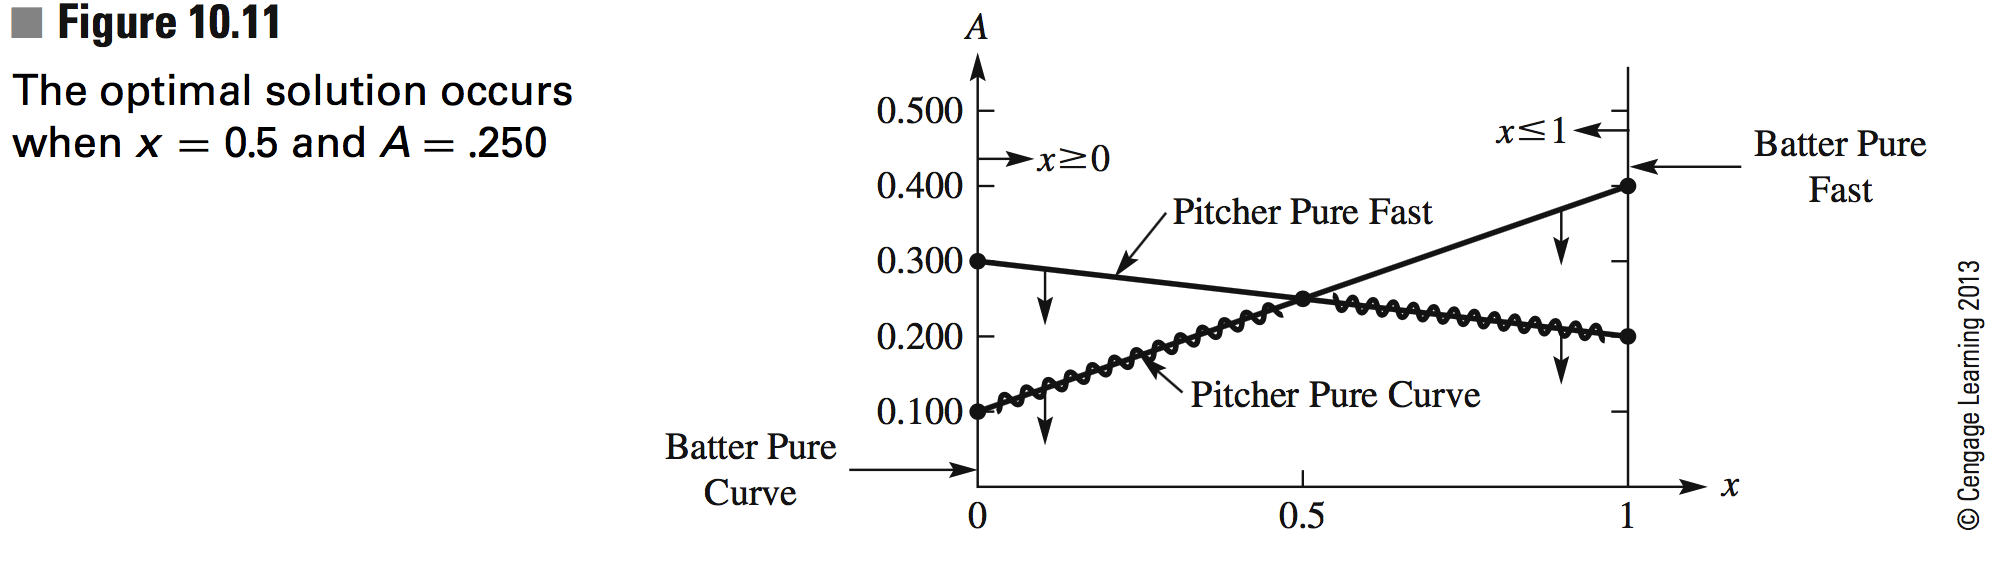
\includegraphics[width=\textwidth{}]{linear.png}
  \end{figure}

\end{frame}

\begin{frame}{决策论:与大自然博弈}
  
  \begin{figure}
    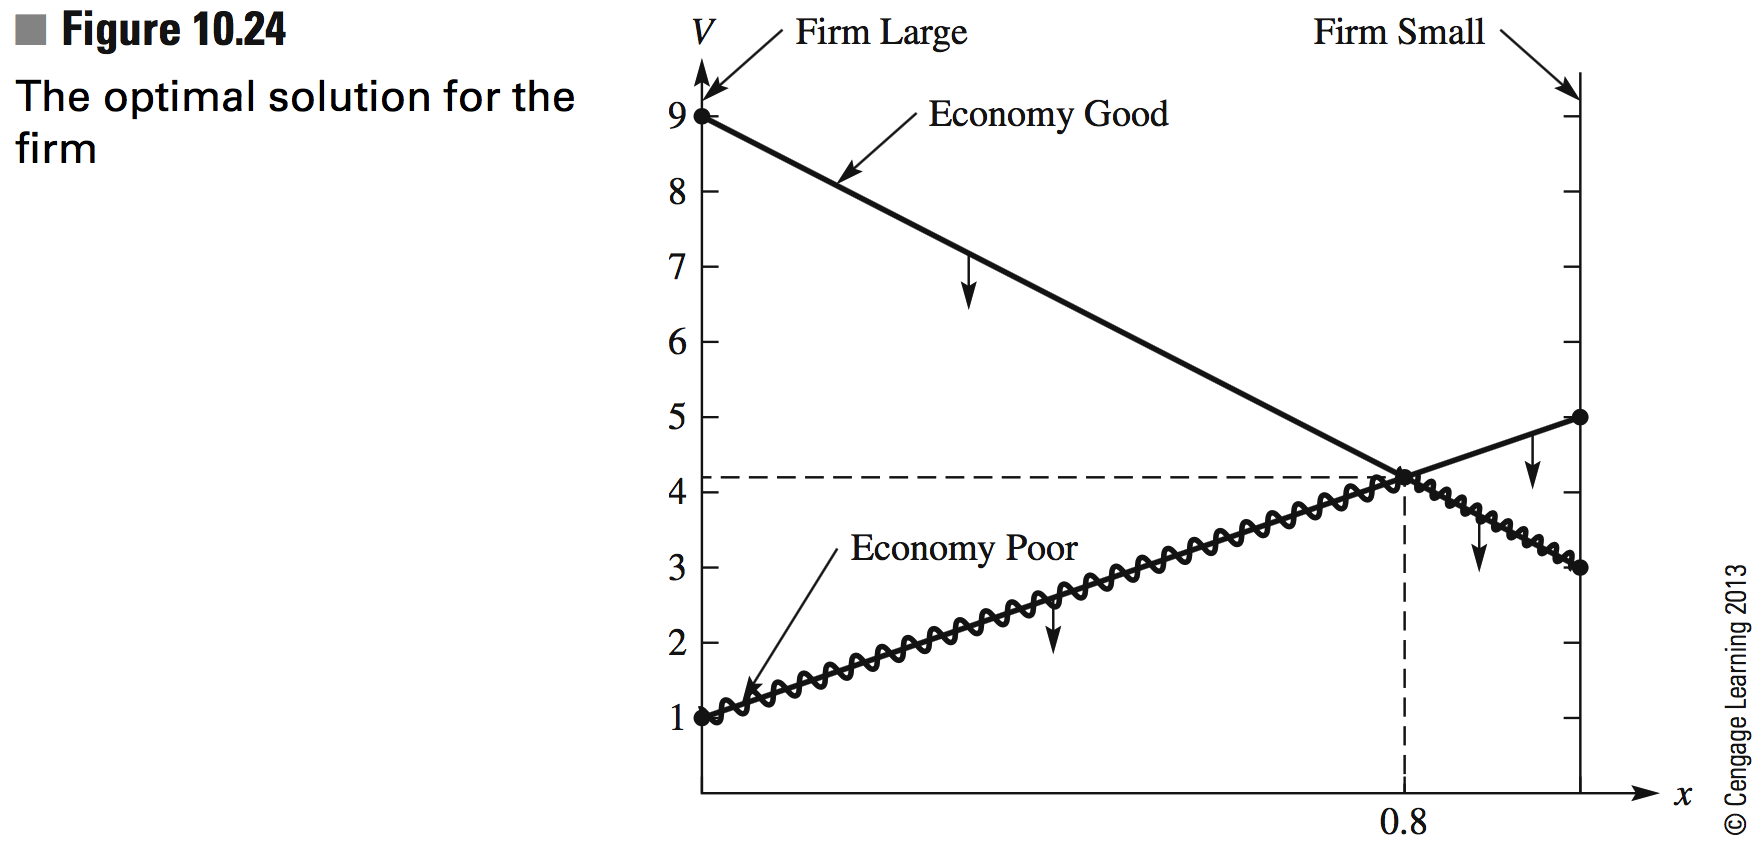
\includegraphics[width=\textwidth{}]{nature.png}
  \end{figure}

\end{frame}

\begin{frame}{2x2 完全冲突博弈的其它简便解法}

  \begin{itemize}
  \item 让对手策略对应的期望值相等
  \item 零头法,也称为William方法
  \end{itemize}
  
\end{frame}

\begin{frame}{部分冲突博弈:经典的两人博弈}
  \begin{itemize}
  \item 囚徒困境
  \item 斗鸡博弈
  \item 性别战
  \end{itemize}
  
\end{frame}


\end{document}

%%% Local Variables: 
%%% TeX-master: t
%%% TeX-engine: xetex
%%% End: 
